 \documentclass[12pt,a4paper,openany,oneside]{report}
\usepackage[utf8]{vietnam}
\usepackage{amsmath, amsthm, amssymb,amsxtra,latexsym,amscd,graphpap,makeidx}
\usepackage{pgf,tikz}
\usepackage{mathrsfs}
\usetikzlibrary{arrows}
\usepackage{float}
\usepackage{listings}
 \usepackage{algorithm}
\usepackage{algpseudocode}
\usepackage{graphicx}
\usepackage{array,tabularx,longtable,multicol,indentfirst,fancyhdr}%
\usepackage[mathscr]{eucal}
\usepackage[top=3.5cm, bottom=3.0cm, left=3.5cm, right=2cm] {geometry}
\usepackage{fancybox}
\usepackage{dirtree}


%==================================  
\newtheorem{dl}{Định lý}[section]
\newtheorem{dn}[dl]{Định nghĩa} 
\newtheorem{bt}[dl]{Bài toán} 
\newtheorem{btp}[dl]{Bài tập} 
\newtheorem{bta}[dl]{Bài} 
\newtheorem{bai}[dl]{Bài}
\newtheorem{tc}[dl]{Tính chất} 
\newtheorem{md}[dl]{Mệnh đề} 
\newtheorem{bd}[dl]{Bổ đề} 
\newtheorem{hq}[dl]{Hệ quả} 
\newtheorem{nx}[dl]{Nhận xét} 
\newtheorem{cy}[dl]{Chú ý} 
\newtheorem{vd}[dl]{Ví dụ} 
\renewcommand{\chaptername}{Chương}
\renewcommand\bibname{Tài liệu tham khảo}
%.....................................

\newcommand{\bpr}{\begin{proof}}
\newcommand{\epr}{\end{proof}}

 

%-----------------------------------------------
\def\en{\enskip}
\def\n{\noindent}
\def\m{\medskip}
\def\en{\enskip}
\def\m{\medskip}
\def\n{\noindent}
\def\Re{\mbox{Re }}
\def\Im{\mbox{Im }}
\def\hcm{\hfill $\square$\\}
\def\imotn{i = 1, 2, \ldots, n}
\def\ii{\item}


\def\N{\mathbb{N}}
\def\Z{\mathbb{Z}}
\def\R{\mathbb{R}}
\def\Q{\mathbb{Q}}
\def\C{\mathscr{C}}  
\def\K{\mathbb{K}}  
\def\F{\mathbb{F}}  
\def\L{\mathbb{L}} 
\DeclareMathOperator{\ord}{ord}

\allowdisplaybreaks
\newenvironment{giai}{\noindent{\em \textit{Giải}. }}{\hfill $\square$}

%%%%%%%%%%%%%%%%%%%%%%%%%%%% 
 
\makeatletter 
\renewcommand{\ps@plain}{
    \renewcommand{\@oddhead}{\hfil{\thepage}\hfil}
    \renewcommand{\@evenhead}{\@oddhead}
    \renewcommand{\@oddfoot}{\empty}
    \renewcommand{\@evenfoot}{\@oddfoot}   }
\makeatother
\pagestyle{fancy}
\fancyhf{}
\rhead{}
\chead{\normalsize  \thepage}
\lhead{\itshape {\nouppercase{}}}
\renewcommand{\headrulewidth}{0pt}


\begin{document}
\pagenumbering{roman}

\newgeometry{top=2.0cm,bottom=3.0cm,left=3.0cm,right=2.8cm}
\setlength{\fboxrule}{1.5pt}
\thisfancypage{\setlength{\fboxsep}{10pt}\setlength{\shadowsize}{0pt}\doublebox}{}

\begin{titlepage}
\fontsize{14pt}{14pt}\selectfont \baselineskip 0.65cm
\thispagestyle{empty}
\begin{center}
{HỌC VIỆN CÔNG NGHỆ BƯU CHÍNH VIỄN THÔNG}\\
\textbf{\MakeUppercase{KHOA CÔNG NGHỆ THÔNG TIN I}}\\
\centerline{--------------------o0o--------------------}  
\end{center}
 

\begin{figure}[H]
	\begin{center}
		
\includegraphics[width=6cm]{./logo}
	\end{center}
\end{figure} 
 
 
\vspace{0.5cm}
\begin{center}
\textbf{\MakeUppercase{\Large \bf ĐỒ ÁN TỐT NGHIỆP ĐẠI HỌC}}\\ 
\end{center} 

\vspace{1cm}
\begin{center}
	\textbf{\MakeUppercase{ \bf BAO LỒI XẤP XỈ VÀ ỨNG DỤNG TRONG VIỆC PHÁT HIỆN ĐỊNH HƯỚNG VÀ ĐÓNG GÓI ĐỐI TƯỢNG}}\\ 
\end{center} 
\vspace{2cm}


\begin{tabular}{ll}
	{\textbf{\large{Giảng Viên Hướng Dẫn: }}} & {\textbf{\large{TS. Nguyễn Kiều Linh}}} \\
	{\textbf{\large{Sinh viên thực hiện:}}}  & {\textbf{\large{Trần Xuân Độ}}} \\
	{\textbf{\large{Mã sinh viên: }}}  & {\textbf{\large{B19DCCN183}}} \\
	{\textbf{\large{Lớp:}}}   & {\textbf{\large{D19CNPM04}}}\\
	{\textbf{\large{Niên khóa:}}}   & {\textbf{\large{2019-2023}}}\\
	{\textbf{\large{Hệ đào tạo:}}}   & {\textbf{\large{Đại học chính quy}}}
\end{tabular}





\vfill
\begin{center}
{{\bf Hà Nội, 12/2023}}
\end{center}
\end{titlepage}

\newgeometry{top=2.0cm,bottom=3.0cm,left=3.0cm,right=2.8cm}
\setlength{\fboxrule}{1.5pt}
\thisfancypage{\setlength{\fboxsep}{10pt}\setlength{\shadowsize}{0pt}\doublebox}{}

\fontsize{14pt}{14pt}\selectfont \baselineskip 0.65cm
\thispagestyle{empty}
\begin{center}
	{HỌC VIỆN CÔNG NGHỆ BƯU CHÍNH VIỄN THÔNG}\\
	\textbf{\MakeUppercase{KHOA CÔNG NGHỆ THÔNG TIN I}}\\
	\centerline{--------------------o0o--------------------}  
\end{center}


\begin{figure}[H]
	\begin{center}
		
\includegraphics[width=6cm]{./logo}
	\end{center}
\end{figure} 



\vspace{0.5cm}
\begin{center}
	\textbf{\MakeUppercase{\Large \bf ĐỒ ÁN TỐT NGHIỆP ĐẠI HỌC}}\\ 
\end{center} 

\vspace{1cm}
\begin{center}
	\textbf{\MakeUppercase{ \bf Bao lồi xấp xỉ và ứng trong việc phát hiện định hướng và đóng gói đối tượng.}}\\ 
\end{center} 
\vspace{2cm}


\begin{tabular}{ll}
	{\textbf{\large{Giảng Viên Hướng Dẫn: }}} & {\large TS. Nguyễn Kiều Linh}\\
	{\textbf{\large{Sinh viên thực hiện:}}}  & {\large Trần Xuân Độ} \\
	{\textbf{\large{Mã sinh viên: }}}  & {\large B19DCCN183} \\
	{\textbf{\large{Lớp:}}}   & {\large D19CNPM04}\\
	{\textbf{\large{Niên khóa:}}}   & {\large 2019-2023}\\
	{\textbf{\large{Hệ đào tạo:}}}   & {\large Đại học chính quy}
\end{tabular}


\vfill
\begin{center}
	{{\bf Hà Nội, 12/2023}}
\end{center}

%%%%%%%%%%%%%%%

\newpage
\restoregeometry
 \pagestyle{fancy}
\pagenumbering{roman}
 \fontsize{13pt}{13pt}\selectfont \baselineskip 0.75cm 

\tableofcontents

%%%%%%%%%%%%%%%%%%%
\newpage
\begin{center}
	\Large{\textbf{LỜI CẢM ƠN}}\\
\end{center}
\vspace{1cm}
Chân thành cảm ơn cô giáo Nguyễn Kiều Linh, người đã đóng góp không ngừng sức mạnh và sự hiểu biết chuyên sâu, giúp tôi hoàn thành đồ án một cách thành công. Những lời hướng dẫn và sự chia sẻ của cô không chỉ giúp tôi giải quyết các vấn đề khó khăn mà còn mở rộng tầm nhìn và kiến thức của tôi trong lĩnh vực công nghệ thông tin.

Tôi cũng muốn bày tỏ lòng biết ơn đặc biệt đến tác giả của các thư viện code MMROTATE và tác giả bài báo BeyoundBoundingBox, người đã chia sẻ những lời khuyên quý báu qua email. Điều này thực sự là một nguồn động viên lớn, giúp tôi áp dụng những kỹ thuật và giải pháp hiệu quả vào dự án của mình.

Cảm ơn anh Linh, đồng nghiệp tại công ty ESC, vì sự hỗ trợ tận tâm và việc cho mượn máy làm việc. Sự thuận tiện này thực sự đã giúp tôi tiếp cận công nghệ và dữ liệu cần thiết một cách dễ dàng và hiệu quả.

Cuối cùng, xin gửi lời tri ân đến bạn bè, những người đã động viên và hỗ trợ tôi trong suốt quá trình thực hiện đồ án. Sự đoàn kết và tình bạn này thực sự là nguồn động viên mạnh mẽ, giúp tôi vượt qua mọi khó khăn. Cảm ơn mọi người vì tất cả!
\
 \\
 
 \
  \\
 \
  \\
 
\phantom{nnnnnnnnnnnnnnnnnnnnnnnnnnnnnnn}\  {\textit{Hà Nội, tháng 11  năm 2023}} \\
\phantom{nnnnnnnnnnnnnnnnnnnnnnnnnnnnnnnnnnnnnnnnn} {Sinh viên}\\
\phantom{nnnnnnnnnnnnnnnnnnnnnnnnnnnnnnnnnn} \\
\phantom{nnnnnnnnnnnnnnnnnnnnnnnnnnnnnnnnnn} \\ 
\phantom{nnnnnnnnnnnnnnnnnnnnnnnnnnnnnnnnnn} \\ 
\phantom{nnnnnnnnnnnnnnnnnnnnnnnnnnnnnnnnnnnnnnn}   {Trần Xuân Độ}


%%%%%%%%%%%%%%%%%%%%%%%%%%%%



\newpage 
\addcontentsline{toc}{chapter}{\bf  Danh sách hình vẽ} 

\listoffigures

%%%%%%%%%%%%%%%%%%%%%%%%%%%%

\newpage 
\addcontentsline{toc}{chapter}{\bf  Danh sách bảng} 
\listoftables

%%%%%%%%%%%%%%%%%%%%%%%%%%%%
	\newpage
{\addcontentsline{toc}{chapter}{Danh sách các ký hiệu và chữ viết tắt}}

\begin{center}
	{\LARGE
		{\bf Danh mục các ký hiệu và chữ viết tắt}}
\end{center}
\vspace{1.25cm}
{\fontsize{13}{13}\selectfont
	\begin{tabular}{ll}
  CFA &  Convex-hull Feature Adaptation\\
  CIoU & Convex Intersection over Union\\
  RoI & Region of Interest transformer\\
  FPN & Feature Pyramid Network\\
  Conv & Convolution\\
  DCN & Deformable Convolution Network\\
  CCW & Counter Clock Wise\\
  \textit{loc} & localization\\
  \textit{cls} & classification\\
  FL & Focal Loss\\
  CUDNN & CUDA Deep Neural Network\\
  CUDA & Compute Unified Device Architecture
	\end{tabular}
}
\newpage
\pagenumbering{arabic} 
\pagestyle{fancy} 

\chapter*{Mở đầu}
\addcontentsline{toc}{chapter}{\vspace*{-8pt}  Mở đầu} 

Trong nhiều thập kỷ, chúng ta đã chứng kiến quá trình phát triển đáng kể của bài toán nhận diện đối tượng. Đóng góp vào sự phát triển này chính là việc sử dụng mạng học sâu kết hợp với đa dạng các cách biểu diễn đặc trưng, các database có kích thước lớn hơn, và việc đào tạo trước các mô hình để tiết kiệm thời gian và chi phí. Tuy nhiên, phần lớn các bộ phát hiện đối tượng đều gặp phải vấn đề khi biểu diễn các đối tượng quan sát từ trên xuống, có hướng tuỳ ý, hoặc các đối tượng có bố cục khác nhau trong quá trình đào tạo. Vấn đề trở nên nghiêm trọng hơn khi các đối tượng phân bố dày dặc, gây ra hiện tượng răng cưa ở các vùng giao nhau của trường tiếp nhận.


Một trong những giải pháp để phát hiện đối tượng có hướng, đó là sử dụng phương pháp làm giàu đặc trưng/mỏ neo, cung cấp nhiều hơn các đặc trưng để đào tạo các bộ phát hiện. Giải pháp này tuy nhiên lại gây ra sự phức tạp trong tính toán, dễ gây ra sai sót. Một giải pháp khác là định nghĩa bộ biến đổi RoI, áp dụng phép biến đổi không gian RoIs trong khi tiếp tục học các tham số dưới sự giám sát của hộp bao có hướng. Các bộ biến đổi này được cho là linh hoạt, nhạy bén, hoạt động mượt mà, cho phép trường tiếp nhận thích nghi với các đối tượng có hướng. Tuy nhiên, vấn đề về cách điều chỉnh lưới đặc trưng cho đối tượng có bố cục bất kỳ vẫn chưa được giải quyết. Đây chính là nguyên nhân gây ra hiện tượng feature aliasing, xảy ra khi các đối tượng phân bổ dày đặc trong khung hình.


Do đó, ta đề xuất một cách tiếp cận khác: sử dụng phương pháp điều chỉnh các đặc trưng bằng bao lồi (convex-hull) dành cho các đối tượng có hướng và phân bố dày đặc. Mục tiêu để điều chỉnh các đặc trưng nằm trong lưới tích chập thông thường với các đối tượng có bố cục phân bố không đều. Ta xây dựng bố cục đối tượng thành một bao lồi, có lợi thế hơn so với sử dụng bố cục hình chữ nhật, giúp bao phủ toàn bộ đối tượng nhưng giảm thiểu tối đa diện tích vùng nền của đối tượng. Mỗi bao lồi là tập hợp các điểm đặc trưng định nghĩa đường biên của đối tượng, biểu thị tỷ lệ Convex Intersection over Union (CIoU) để các định vị trí đối tượng. Bên trong bao lồi, các đặc trưng khác nhau biểu thị cho sự xuất hiện của các đối tượng được phân loại khác nhau.


Mục tiêu của đồ án là tìm hiểu, nghiên cứu phương pháp phát hiện đối tượng dày đặc có hướng, cụ thể là nghiên cứu phương pháp BeyoundBoundingBox dành cho vấn đề trên. Ngoài ra, đồ án còn tìm hiểu thuật toán phát hiện bao lồi mới, thay thế vào phương pháp trên, kiểm nghiệm và đo lường độ hiệu quả của thuật toán mới này.


Trong đồ án em sẽ tập trung trình bày một số nội dung chính như sau:

\textbf{Chương 1: Giới thiệu bài toán phát hiện, định hướng và đóng gói đối tượng:}
Nội dung chương 1 sẽ khái quát các vấn đề và phương pháp nhận dạng đối tượng, trình bày về các phương pháp liên quan, nguyên lý và cách thức triển khai, giới thiệu sử dụng thuật toán bao lồi xấp xỉ để thực hiện bài toán.


\textbf{Chương 2: Trình bày thuật toán bao lồi xấp xỉ:}
Nội dung của chương 2 sẽ giới thiệu thuật toán, lý thuyết và triển khai thuật toán bằng code C++


\textbf{Chương 3: Thực nghiệm và kết quả:}
Nội dung của chương 3 Áp dụng bao lồi xấp xỉ cho bài toán phát hiện, định hướng và đóng gói đối tượng, cách thức triển khai bộ phát hiện, cách thức thay thế thuật toán.


\textbf{Chương 4: Tổng kết:}
Tổng kết bài toán, tóm tắt những kết quả đã đạt được và còn chưa đạt được. Từ đó đề xuất mục tiêu hướng tới cũng như hướng nghiên cứu, phát triển tiếp theo.



 


\chapter{Giới thiệu bài toán phát hiện, định hướng và đóng gói đối tượng}

Chương 1 đặt vấn đề về bài toán phát hiện đối tượng, trình bày lý thuyết về phương pháp BeyoundBoundingBox.



\section{Giới thiệu}
Trong bài toán phát hiện đối tượng, việc định vị và phát hiện đối tượng dày đặc vẫn còn là một vấn đề thách thức do vấn đề đặc trưng răng cưa (feature aliasing), tức là các pi. Có các giải pháp đã được sử dụng: làm giàu các đặc trưng (enhance features) và sử dụng anchors. Nhược điểm của các phương pháp này: làm cho cấu trúc mạng trở nên phức tạp hơn, tăng thời gian huấn luyện (training) và suy luận (inference). Một phương pháp khác đó là sử dụng biến đổi RoI, nhưng phương pháp này không thích ứng tốt với các đối tượng có hướng bất kỳ, đặc biệt đối với các đối tượng xuất hiện dày đặc trong hình ảnh.


\begin{figure}[ht!]
	\begin{center}
		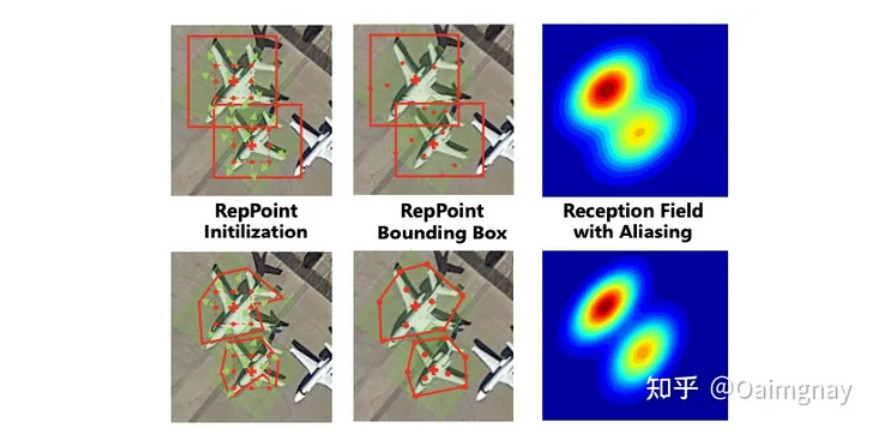
\includegraphics[width=400px]{./compare_cfa_with_other.JPG}
		\caption{Minh hoạ vấn đề. (Bên trên) Sử dụng cách biểu diễn dạng hộp, so với cách biểu diễn bao lồi (Bên dưới), hiện tương răng cưa đã được xử lý}
		\label{fig_dhandang1}
	\end{center}
\end{figure} 


Để giải quyết các vấn đề trên, một phương pháp đã được đưa ra: phương pháp thích ứng bao lồi (convex-hull feature adaptation-CFA). CFA được thực hiện dựa trên phương pháp biểu diễn bao lồi, định nghĩa một tập các điểm đặc trưng, giới hạn phạm vi của đối tượng mục tiêu sử dụng chỉ số CIoU. CFA đạt được sự phân bổ đặc trưng tối ưu nhờ vào việc xây dựng tập bao lồi và phân chia linh hoạt các bao lồi thành các bao lồi âm và bao lồi dương. CFA cũng xem xét sự chồng chéo nhau giữa bao lồi dự đoán và bao lồi thực tế, phạt các bao lồi được dùng chung bởi nhiều đối tượng, giảm thiểu hiện tượng đặc trưng răng cưa (feature aliasing), đạt được sự thích ứng đặc trưng tối ưu. Nó cũng đạt được kết quả tốt nhất khi thử nghiệm trên tập dữ liệu DOTA và SKUR110KR.

Phương pháp CFA được chia làm 2 giai đoạn thực hiện:
\begin{itemize}
	\item Giai đoạn 1: tạo tập bao lồi và ước lượng sơ bộ bố cục của bao lồi.
	\item Giai đoạn 2: chỉnh sửa bao lồi sao cho phù hợp với các đối tượng phân bổ dày đặc.
\end{itemize}

\begin{figure}[ht!]
	\begin{center}
		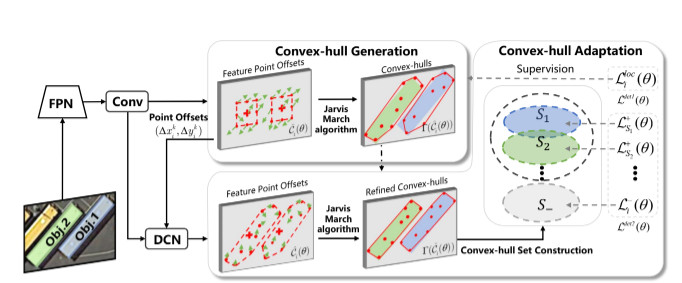
\includegraphics[width=450px]{./work_flow_cfa.JPG}
		\caption{Biểu đồ luồng quy trình thực hiện của bộ phát hiện CFA.}
		\label{work_flow_cfa}
	\end{center}
\end{figure} 

\section{Xây dựng tập bao lồi đầu tiên}
Việc biểu diễn bằng khung hình chữ nhật do bao lồi sinh ra làm giảm khả năng biểu diễn đối tượng. Vì thế phương pháp CFA đã đề xuất biểu diễn phạm vi của đối tượng bằng bao lồi. Mỗi bao lồi là một tập hợp các điểm thoả mãn công thức:

\begin{align} \label{convex_hull_definition}
		C_i=\left\{\left(x_i^k, y_i^k\right)\right\}_i^{k=1 \ldots K}
\end{align}
Trong đó: $C_i$ là bao lồi thứ i, $\left(x_i^k, y_i^k\right)$ là điểm nằm trên bao lồi thứ k, k là chỉ số của điểm đặc trưng, $K = 9$ tương ứng với 9 điểm được khởi tạo của bao lồi.

\begin{figure}[ht!]
	\begin{center}
		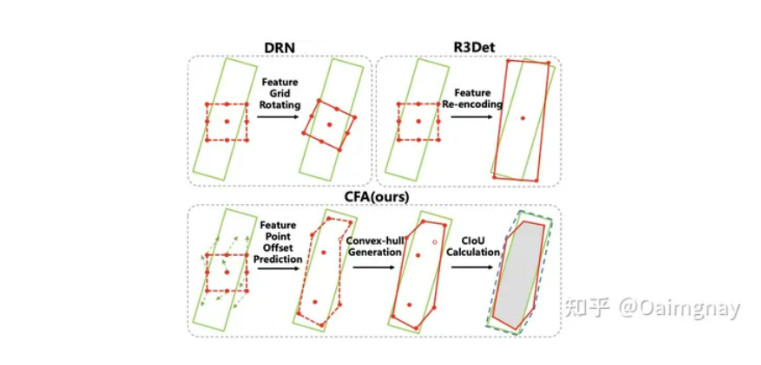
\includegraphics[width=445px]{./compare_convex-hull_with_rectangle.jpg}
		\caption{So sánh biểu diễn hộp có hướng (bên trên) so với biểu diễn bao lồi (ở dưới).}
	\end{center}
\end{figure} 


Việc huấn luyện có thể xem như là quá trình dự đoán độ lệch (offset), trong khi hệ số CIoU cần được tối đa hoá để đạt được so khớp tối ưu nhất. Đây là phương pháp sử dụng phép toán tích chập để dự đoán độ lệch:
$\left(\Delta x_i^k, \Delta y_i^k\right)$
với từng điểm đặc trưng, sau trả về một bản đồ độ bù cho các đặc trưng
$O \in R^{H \times W \times W}$ ($H, W, C$ lần lượt tương ứng với chiều dài, chiều rộng và số lượng kênh của bản đồ đặc trưng):
\begin{align} \label{convex_hull_learn_offset}
	\hat{\mathcal{C}}_i(\theta) \leftarrow\left\{\left(x_i^k+\Delta x_i^k(\theta), y_i^k+\Delta y_i^k(\theta)\right)\right\}_i^{k=1 \ldots K}
\end{align}

Trong đó: $\theta$ biểu thị là các tham số của mạng. Việc dự đoán offset sẽ thực hiện theo công thức trên.

\section{Tích chập biến dạng}
Tích chập biến dạng (Deformable convolution - DCN) \cite{DCN} là dạng tích chập mà vị trí thực hiện tích chập bị biến dạng, không giống tích chập truyền thống là dạng lưới $N\mathrm{x}N$. Ưu điểm của phương pháp này giúp trích xuất các đặc trưng mong muốn được chính xác hơn, lấy mẫu được ở những vị trí đa dạng hơn (Phép tích chập truyền thống chỉ có thể trích xuất các đặc trưng trên một khung hinh chữ nhật).(Hình \ref{so_sanh_tich_chap_thong_thuong_deformable})

\begin{figure}[ht!]
	\begin{center}
		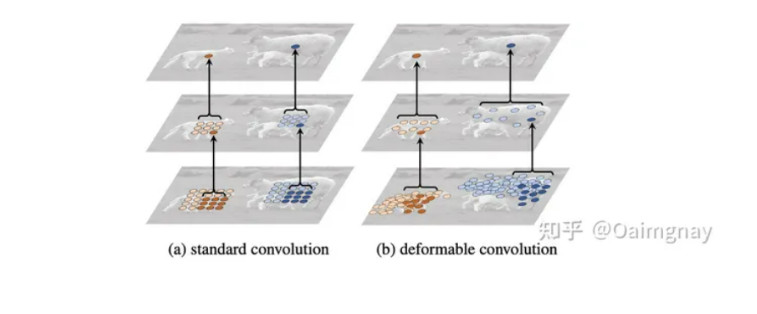
\includegraphics[width=445px]{./compare_normal_with_deformable_convolution.jpg}
		\caption{So sánh tích chập thông thường và tích chập biến dạng.}
		\label{so_sanh_tich_chap_thong_thuong_deformable}
	\end{center}
\end{figure} 

Phép tích chập biến dạng thực ra là thêm phần bù cho các điểm tích chập lấy mẫu. (Hình \ref{offset_deformable_convolution})

\begin{figure}[ht!]
	\begin{center}
		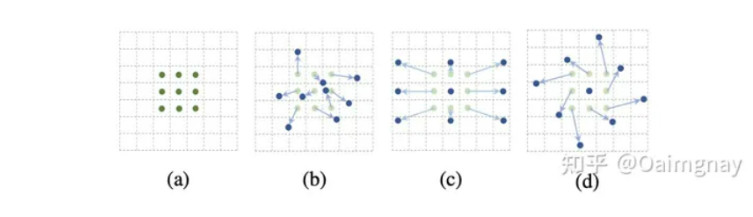
\includegraphics[width=445px]{./feature_offset_type.jpg}
		\caption{Các phép biến đổi tích chập biến dạng khác nhau
		}
		\label{offset_deformable_convolution}
	\end{center}
\end{figure} 

\begin{figure}[ht!]
	\begin{center}
		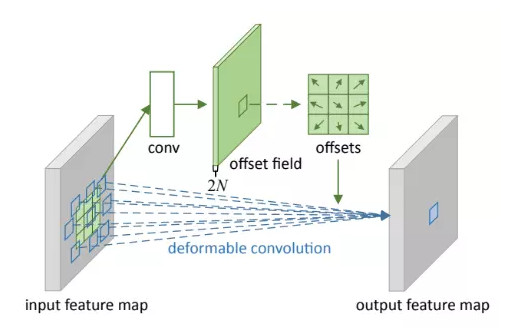
\includegraphics[width=400px]{./deformable_process.jpg}
		\caption{Quá trình thực hiện tích chập biến dạng.}
		\label{deformable_process}
	\end{center}
\end{figure} 


Cho đầu vào là một bản đồ đặc trưng, giả sử phép tích chập là 3x3. Để học được phần bù, định nghĩa một lớp tích chập 3x3 khác, chiều của đầu ra là kích thước của bản đồ đặc trưng ban đầu, số kênh = $2N$. (Hình \ref{deformable_process}) Tiếp theo thực hiện tích chập biến dạng, dựa trên độ bù của các phần đã được tính trước đó, sau đó thực hiện phép tích chập như thông thường.
\section{Thuật toán Convex Approximation}
Sau khi học được phần bù, việc hoàn thành cập nhật các điểm đặc trưng của bao lồi được thực hiện bởi thuật toán Outer Convex Approximation, hoặc Inner Convex Approximation (cả hai thuật toán đều sử dụng $\delta$ = 0, không lấy bao lồi xấp xỉ). Bao lồi nhỏ nhất phù hợp điều kiện sẽ được chọn ra sau mỗi lần lặp.
\subsection{Thuật toán Outer Convex Approximation}
\begin{figure}[ht!]
	\begin{center}
		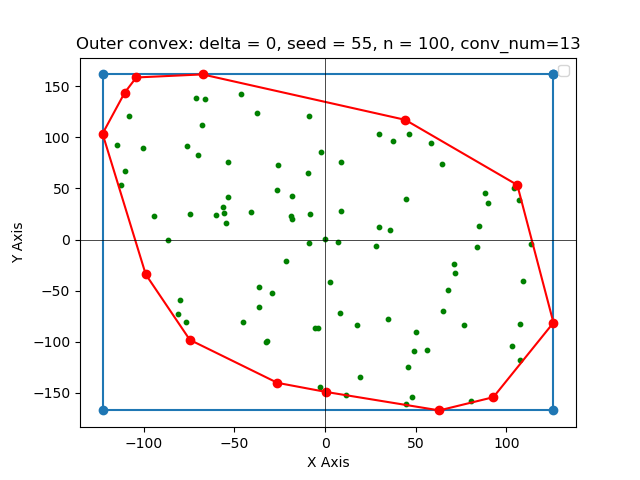
\includegraphics[width=350px]{./outer_convex_approximation_brief.png}
		\caption{Minh họa thuật toán Outer Convex Approximation.}
		\label{outer_convex_approximation_brief}
	\end{center}
\end{figure} 
Tóm tắt thuật toán Outer Convex Approximation (Hình \ref{outer_convex_approximation_brief}): Xuất phát từ một hình chữ nhật nhỏ nhất bao quanh tất cả các điểm (màu xanh dương), thuật toán duyệt lần lượt các đỉnh được chọn, xác định hướng cực đại (direction) nhờ hai điểm liền trước (predecessor) và điểm liền sau (successor), để quyết định việc lấy thêm đỉnh mới cho bao lồi. Kết quả cuối cùng sẽ là hình chữ nhật được cải thiện dần thành bao lồi (màu đỏ) phù hợp với toàn bộ tập điểm. 
\subsection{Inner Convex Approximation}
\begin{figure}[ht!]
	\begin{center}
		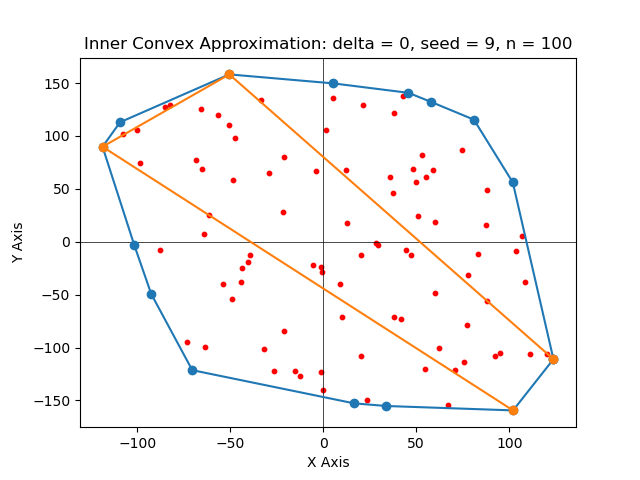
\includegraphics[width=350px]{./inner_convex_brief.png}
		\caption{Minh họa thuật toán Inner Convex Approximation với đầu vào gồm 100 điểm ngẫu nhiên.}
		\label{inner_convex_brief}
	\end{center}
\end{figure} 
Tóm tắt thuật toán (Hình \ref{inner_convex_brief}): Xuất phát từ hình tứ giác ban đầu (màu cam), ứng với mỗi cạnh sẽ chọn các điểm phù hợp trong tập các điểm phía trên cạnh đó để mở rộng tứ giác. Sau cùng khi không còn điểm nào nằm phía trên các cạnh, thuật toán sẽ kết thúc, trả về bao lồi (màu xanh lam).
\section{Đinh nghĩa công thức Convex Intersection over Union (CIoU)}
Dựa vào mỗi bao lồi dự đoán, có thể tính toán được hàm mất mát vị trí và phân lớp của một đối tượng. Công thức CIoU giữa bao lồi dự đoán thứ $i$:  $C_i(\theta)$ và hộp bao thật sự $\mathcal{B}_j$ của đối tượng thứ $j$ được tính như sau:

\begin{align} \label{CioU_fomular}
	\operatorname{CIoU}\left(\mathcal{C}_i(\theta), \mathcal{B}_j\right)=\frac{\left|\mathcal{C}_i(\theta) \cap \mathcal{B}_j\right|}{\left|\mathcal{C}_i(\theta) \cup \mathcal{B}_j\right|}-\frac{\left|\mathcal{R}_j \backslash\left(\mathcal{C}_i(\theta) \cup \mathcal{B}_j\right)\right|}{\left|\mathcal{R}_j\right|}
\end{align}
Trong đó: $\mathcal{R}_j$ là hợp của hai đa giác, tức là đa giác nhỏ nhất có thể bao quanh  $C_i(\theta)$ và $\mathcal{B}_j$.
\section{Hàm mất mát}
Theo công thức \ref{CioU_fomular}, hàm mất mát vị trí CIoU được định nghĩa là:
\begin{align} \label{cong_thuc_ham_loss_CIoU}
	\mathcal{L}_i^{l o c}(\theta)=1-\operatorname{CIoU}\left(\mathcal{C}_i(\theta), \mathcal{B}_j\right)
\end{align}
Cho $f_i^{k}(\theta)$ là đặc trưng của điểm thứ $k$, bao lồi đặc trưng $f_i(\theta)$ được tính bởi tổng có trọng số của tất cả các điểm đặc trưng trên bao lồi dự đoán $\mathcal{C}_i(\theta)$, tức là bằng công thức: $f_i(\theta) = \sum_{k}m w_i^k.f_i^k(\theta)$, trong đó, $w_i^k$ biểu thị các trọng số đặc trưng có thể học được từ tích chập biến dạng (DCN). Dựa vào bao lồi đặc trưng, điểm dự đoán $S_i(\theta)$ của bao lồi dự đoán $C_i(\theta)$ được tính bởi phép tích chập, hàm mất mát phân loại của bao lồi dự đoán $C_i(\theta)$ tương ứng với $B_j$ được định nghĩa là:
\begin{align} \label{loss_classification}
	\mathcal{L}_i^{c l s}(\theta)=\mathrm{FL}\left(S_i(\theta), Y_j\right)
\end{align}
ở đây $Y_j$ biểu thị là nhãn nhị phân thật sự (ground-truth) và FL() ở đây là hàm mất mát Focal (Focal loss). Kết quả có được là hàm mất mát dành cho bao lồi dương: 
\begin{align} \label{loss_function_positive_convex}
	\mathcal{L}_i^{+}(\theta)=\mathcal{L}_i^{c l s}\left(\mathcal{S}_i(\theta), Y_j\right)+\lambda \mathcal{L}_i^{l o c}\left(\mathcal{C}_i(\theta), \mathcal{B}_j\right)
\end{align}
Hàm mất mát \ref{loss_function_positive_convex} là tổng của hàm mất mát vị trí \ref{cong_thuc_ham_loss_CIoU} và hàm mất mát phân loại \ref{loss_classification}.
Hàm mất mát dành cho bao lồi âm là:

\begin{align} \label{loss_negative_convex}
	\mathcal{L}_i^{-}(\theta)=\mathcal{L}_i^{c l s}\left(\mathcal{S}_i(\theta), Y_j\right)
\end{align}
Ngoài ra, trong quá trình huấn luyện (Hình \ref{work_flow_cfa}), vì các bao lồi được ban đầu chỉ được sinh ra bằng cách tối ưu CIoU, một hàm loss cần được định nghĩa cho việc giám sát:
\begin{align} \label{loss_det_1}
	\mathcal{L}^{\operatorname{det} 1}(\theta)=\frac{1}{J} \sum_i \mathbb{I}_{\left(x_i, y_i\right)} \mathcal{L}_i^{l o c}(\theta)
\end{align}
Nhìn chung, trong giai đoạn đầu tiên của việc sinh bao lồi, hàm mất mát $L^{\operatorname{det} 1}$ bên trên là hàm cần được quan tâm. Trong giai đoạn 2, hai hàm mất mát phân lớp (\ref{loss_negative_convex} và \ref{loss_function_positive_convex}) sẽ được sử dụng để phân loại bao lồi
\section{Thích ứng bao lồi}
Phương pháp biểu diễn bằng bao lồi giúp định vị đối tượng ở bất kỳ hình dạng nào, tuy nhiên vẫn có một vấn đề, làm thế nào để định vị một cách chính xác các đối tượng dày đặc, đặc biệt là các đối tượng có đặc trưng răng cưa. Vì vậy bộ phát hiện CFA đã đề xuất một phương pháp thích ứng mới để tinh chỉnh các bao lồi sinh ra ở giai đoạn 1 để đạt được vị trí chính xác hơn và phân lớp hiệu quả hơn.
\subsection{Xây dựng tập các bao lồi}
Bộ phát hiện cho xây dựng một tập các bao lồi với mỗi đối tượng, để một đối tượng mục tiêu có thể khớp với nhiều bao lồi phù hợp để cùng nhau tối ưu các đặc trưng của các đối tượng dày đặc.

\begin{figure}[ht!]
	\begin{center}
		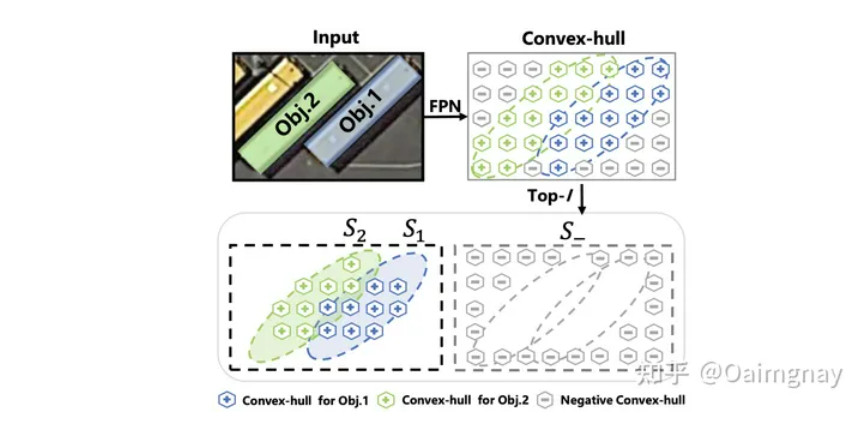
\includegraphics[width=445px]{./construction_convex_hull_set.jpg}
		\caption{Minh họa xây dựng tập các bao lồi để biểu diễn các đối tượng, đặc biệt với những đối tượng phân bổ dày đặc.}
		\label{fig_dhandang1}
	\end{center}
\end{figure} 
Với mỗi một đối tượng, ý tưởng xây dựng tập bao lồi tương ứng là: theo như hệ số CIoU giữa bao lồi dự đoán và bao lồi thực tế, chọn I bao lồi đứng đầu là ứng cử viên cho bao lồi dương để xây dựng tập các bao lồi. Ngoài ra cũng có thể xây dựng tập bao lồi sử dụng ngưỡng CIoU xác định bằng thực nghiệm. Các bao lồi còn lại không thuộc vào bất kỳ tập bao lồi nào sẽ được gộp lại thành tập bao lồi âm $S$.
\begin{align} \label{construct_convex_hull_set}
\mathcal{L}_{S_j}^{+}(\theta)=\frac{1}{\left|S_j\right|} \sum_{i \in S_j} \omega_i \mathcal{L}_i^{+}(\theta)
\end{align}
Khi nhiều đối tượng tập hợp lại cùng nhau, không phải tất cả các bao lồi nằm trong tập bao lồi đều phù hợp với đối tượng, và các bao lồi có đặc trưng răng cưa sẽ phải được phân loại thành tập các bao lồi âm. Cùng thời điểm đó, các bao lồi được chia sẻ bởi nhiều đối tượng phải phải có độ tin cậy thấp hơn.
\subsection{Chiến lược phân đoạn tập các bao lồi}
Để giải quyết vấn đề đặc trưng răng cưa ở các đối tượng dày đặc, bộ phát hiện CFA đề xuất chiến lược phân đoạn tập các bao lồi để đánh giá động các mẫu bao lồi âm và mẫu dương, chuyển đổi trọng số $\omega_i$ thành $f\left(L_i^{+}(\theta)\right)$. Sau khi thay thế, được công thức sau:
\begin{align} \label{loss_positive_convert}
	\mathcal{L}_{s_j}^{+}(\theta)=\frac{1}{\left|S_j\right|} \sum_{i \in S_j} f\left(\mathcal{L}_i^{+}(\theta)\right) \mathcal{L}_i^{+}(\theta)
\end{align}
Trong đó: $f$ là hàm lỗi đơn điệu giảm phân phối Gaussian: $f\left(x\right) = 1.0 - \frac{2}{\sqrt{\pi}}\int_0^xe^{-t^2}$, có nghĩa là giá trị mất càng nhỏ, độ tin cậy càng cao.

\begin{figure}[ht!]
	\begin{center}
		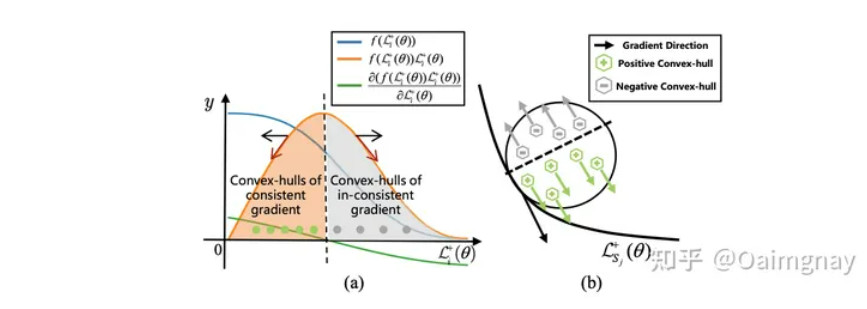
\includegraphics[width=445px]{./gaussian_gradient.jpg}
		\caption{Phân chia tập bao lồi theo hướng dẫn của nguyên tắc nhất quán độ dốc.}
		\label{gradient_consistentcy_illustration}
	\end{center}
\end{figure} 
Nguyên tắc phân chia tập bao lồi là nguyên tắc nhất quá độ dốc. Bằng cách lấy đạo hàm của công thức công thức \ref{loss_positive_convert}, ta có được:
\begin{align} \label{gradient_of_loss}
	 \frac{\partial \mathcal{L}_{s_j}^{+}(\theta)}{\partial \theta}=\frac{1}{\left|S_j\right|} \sum_{i \in S_j} \frac{\partial\left(f\left(\mathcal{L}_i^{+}(\theta)\right) \mathcal{L}_i^{+}(\theta)\right)}{\partial \mathcal{L}_i^{+}(\theta)} \frac{\partial \mathcal{L}_i^{+}(\theta)}{\partial \theta}
\end{align}
Tiêu chí để thực hiện phân đoạn tập các bao lồi là: đạo hàm của mỗi một bao lồi dương $\frac{\partial L_i^{+}(\theta)}{\partial \theta}$ yêu cầu đạo hàm của toàn bộ tập bao lồi $\frac{\partial L_{S_j}^{+}(\theta)}{\partial \theta}$ là nhất quán. Điều này có nghĩa là: bao lồi nào có độ dốc không nhất quán được xem là bao lồi âm, tức là những bao lồi này sẽ dẫn đến hiện tượng răng cưa đặc trưng. Xem xét công thức \ref{gradient_of_loss}, nếu $\frac{\partial\left(f\left(L_i^{+}(\theta)\right) L_i^{+}(\theta)\right)}{\partial L_i^{+}(\theta)}$ mang giá trị dương, thì bao lồi $C_i$ được xếp là bao lồi dương, hoặc ngược lại bao lồi sẽ là âm. Xem xét hình \ref{gradient_consistentcy_illustration}, khi sắp xếp các giá trị mất mát  $\frac{\partial L_i^{+}(\theta)}{\partial \theta}$ theo thứ tự tăng dần, $f\left(\partial L_i^{+}(\theta)\right) L_i^{+}(\theta)$ (đường màu cam) là một hàm lồi hướng lên với một cực trị duy nhất, trong khi đường  $\frac{\partial\left(f\left(L_i^{+}(\theta)\right) L_i^{+}(\theta)\right)}{\partial L_i^{+}(\theta)}$ (màu xanh lục) chia các bao lồi thành tập các bao lồi dương $S_j$ và tập bao lồi âm $S\_$.

Cùng thời điểm đó, để xử lý đặc trưng răng cưa, tác giả cũng giới thiệu hệ số chống đặc trưng răng cưa:
\begin{align}\label{FAA_fomular}
	p_i = \gamma\dot{\frac{\mathrm{CIoU}(\mathcal{C}_i, \mathcal{B}_j)}{\sum_{m=1}^{M}\mathrm{CIoU}\left(\mathcal{C}_i, \mathcal{B}_j\right)}}
\end{align}
Hệ số này thể hiện mức độ mà một đối tượng thuộc về một đối tượng duy nhất, khi nó chồng lên M đối tượng khác. $\gamma$ là hệ số chống đặc trưng răng cưa.
Hàm mất mát được cập nhật thành: 

\begin{align}\label{loss_update}
	\mathcal{L}_{s_j}^{+}(\theta)=\frac{1}{\left|S_j\right|} \sum_{i \in S_j} p_i f\left(\mathcal{L}_i^{+}(\theta)\right) \mathcal{L}_i^{+}(\theta)
\end{align}
Giai đoạn 2 của quá trình tối ưu được điều khiển bởi hàm mất mát trên tập bao lồi, hàm này được xác định bằng cách kết hợp hàm mất mát phân loại và hàm mất mát vị trí:
\begin{align} \label{loss_det_2}
	\begin{aligned}
		\mathcal{L}^{\operatorname{det} 2}(\theta)= & \frac{1}{J} \sum_{j=1}^J \frac{1}{\left|S_j\right|} \sum_{i \in S_j} p_i f\left(\mathcal{L}_i^{+}(\theta)\right) \mathcal{L}_i^{+}(\theta) \\
		& +\frac{1}{\left|S_{-}\right|} \sum_{i \in S_{-}} \mathcal{L}_i^{-}(\theta)
	\end{aligned}
\end{align}

Hàm mất mát này xem xét sự tương ứng về đặc trưng của nhiều đối tượng, tiến hành phạt các bao lồi được chia sẻ bởi nhiều đối tượng, và giảm thiểu đặc trưng răng cưa để đạt được thích ứng đặc trưng tối ưu. Cuối cùng hàm mất mát của toàn bộ bộ phát hiện CFA là: 
\begin{align} \label{final_loss_CFA}
	L^{\operatorname{det} 1}(\theta)+L^{\operatorname{det} 2}(\theta)
\end{align}

\chapter{Thuật toán tính bao lồi xấp xỉ}
Thuật toán tìm bao lồi xấp xỉ nhận đầu vào là một tập các điểm ngẫu nhiên, đầu ra trả về một tập điểm biểu diễn một bao lồi bao quanh tất cả các điểm còn lại. Với ngưỡng $\delta$ tuỳ chỉnh, sẽ cho ra được dạng bao lồi khác nhau.
\section{Outer convex approximation}
Cho tập X được định nghĩa như sau:
\begin{align} \label{ct2.1} 
	X:=\left\{x_1, x_2, \ldots, x_n\right\} \subset \mathbb{R}^2
\end{align}
Giả sử không mất tính tổng quát rằng:
\begin{align} \label{ct2.2} 
	x_1, x_2, \ldots, x_n  \text{ không cùng nằm trên cùng một đường thẳng.}
\end{align}
Ta viết tất cả các vector thành dạng vector hàng, những vector này sẽ có chuyển vị của chúng được ký hiệu bởi chỉ số trên $T$, và sử dụng chỉ số trên để chỉ định các thành phần của chúng, ví dụ: $x = \left(x^1, x^2\right)\in\mathbb{R}^2$. Cho $x, x'\in\mathbb{R}^2$, chứng tỏ:
\begin{equation}\label{ct2.3}
	\begin{aligned}
		& {\left[x, x^{\prime}\right]:=\left\{(1-\lambda) x+\lambda x^{\prime} \mid \lambda \in[0,1]\right\}} \\
		& \left(x, x^{\prime}\right):=\left\{(1-\lambda) x+\lambda x^{\prime} \mid \lambda \in(0,1)\right\}
	\end{aligned}
\end{equation}

Cho $X$ thỏa mãn (\ref{ct2.1}) - (\ref{ct2.2}) và $\delta \geq 0$, trong phần này ta muốn tìm một bao lồi xấp xỉ của $X$, ký hiệu:
\begin{align}\label{ct2.4}
	\text{Đa giác lồi }\mathcal{P}^{outer} \text{thỏa mãn bao lồi }X\subset\mathcal{P}^{outer}
\end{align}
sao cho:
\begin{align}\label{ct2.5}
	dist_H\left(conv\ X, \mathcal{P}^{outer}\right) \leq \delta
\end{align}
$\mathcal{P}^{outer}$ đươc xác định bởi:
\begin{align}\label{ct2.6}
	\mathcal{P}^{outer} := \{x\in\mathbb{R}^2 |\ dx^T \leq \beta_d\ \text{ với tất cả d} \in D\}
\end{align}
Trong đó $D \subset \mathbb{R}^2$ biểu thị tập các hướng tối đa, $\beta_d \in \mathbb{R}$ biểu thị ngưỡng tương ứng với hướng $d \in D$. Với tập D cho trước, $\mathcal{P}^{outer}$ là bao lồi xấp xỉ phù hợp nhất chứa $X$ nếu như:
\begin{equation}\label{ct2.7}
	\beta_d:=\max _{x \in X}\ d x^T \text{với tất cả d }\in D
\end{equation}
Cho P là tập các đỉnh của $\mathcal{P}^{outer}$.\\
Ta bắt đầu quá trình xác định bao lồi xấp xỉ ngoài với hình chữ nhật nhỏ nhất chứa $X$, có chứa cạnh song song với trục tung và trục hoành. Theo công thức (\ref{ct2.5}) - (\ref{ct2.6}), hình chữ nhật $\mathcal{P}^{outer}$ được xác định như sau:
\begin{align}\label{ct2.8}
	D:=\{(1, 0), (0, 1), (-1, 0), (0, -1)\}
\end{align}
và:
\begin{equation}\label{ct2.9}
	\begin{aligned}
		& \beta_{(1,0)}:=\max \left\{x^1 \mid\left(x^1, x^2\right) \in X\right\}, \\
		& \beta_{(0,1)}:=\max \left\{x^2 \mid\left(x^1, x^2\right) \in X\right\}, \\
		& \beta_{(-1,0)}:=\max \left\{-x^1 \mid\left(x^1, x^2\right) \in X\right\}, \\
		& \beta_{(0,-1)}:=\max \left\{-x^2 \mid\left(x^1, x^2\right) \in X\right\} .
	\end{aligned}
\end{equation}
Theo công thức (\ref{ct2.2}) ta có:

\begin{center}
	$\beta_{(-1, 0)} \textless \beta_{(1, 0)}$ \text{ và } $\beta_{(0, -1)} \textless \beta_{(0, 1)}$
\end{center}
Vì vậy, $\mathcal{P}^{outer}$ là một hình chữ nhật phù hợp với 4 đỉnh phân biệt, có tập đỉnh là:
\begin{align}\label{ct2.10}
	P := \{r_1, r_2, r_3, r_4\}
\end{align}
Trong đó:
\begin{equation}\label{ct2.11}
	\begin{aligned}
		& r_1:=\left(\beta_{(1,0)}, \beta_{(0,1)}\right), \\
		& r_2:=\left(\beta_{(-1,0)}, \beta_{(0,1)}\right), \\
		& r_3:=\left(\beta_{(-1,0)}, \beta_{(0,-1)}\right), \\
		& r_4:=\left(\beta_{(1,0)}, \beta_{(0,-1)}\right) .
	\end{aligned}
\end{equation}
Trong các bước xấp xỉ tiếp theo, xây dựng đa giác $\mathcal{P}^{outer}$ được cải thiện dần dần như sau:

$\text{Với mỗi }p \in P, \text{lấy } p^{-} \in P \text{ và } p^{+} \in P \text{ lần lượt là}$
\begin{align} \label{ct2.12}
\text {điểm liền trước ngược chiều kim đồng hồ và điểm liền sau của } p.
\end{align}
Xét công thức sau:
\begin{equation}\label{ct2.13}
	\begin{array}{lcl}
		d_{p}^T &:=& \|p^+ - p^-\|^{-1}\, R \, (p^+ - p^-)^T, \\
		\beta_{d_{p}} &:=& \max\{d_{p}\, x^T \mid x \in X\},
	\end{array}
\end{equation}
Trong đó:
\begin{equation}\label{ct2.14}
	R := \begin{pmatrix}
		0 & -1 \\
		1 & 0
	\end{pmatrix}
\end{equation}
là ma trận xoay ngược chiều theo hướng kim đồng hồ với góc xoay $\pi/2$. Vì $R$ là ma trận xoay, ta có:
\begin{equation}\label{ct2.15}
	\|d_{p}\| = \|p^+ - p^-\|^{-1}\, \|(p^+ - p^-) R^T\| = \|p^+ - p^-\|^{-1}\, \|p^+ - p^-\| = 1.
\end{equation}
Có hai trường hợp xảy ra khi ta thêm các ràng buộc tuyến tính sau vào định nghĩa của $\mathcal{P}^{outer}$ trong công thức (\ref{ct2.6}):
\begin{equation}\label{ct2.16}
	d_p\, x^T \leq \beta_{d_p}.
\end{equation}

Trường hợp 1, nếu:
\begin{equation}\label{ct2.17}
	\beta_{d_p} = d_p\, p^+
\end{equation}
thì công thức (\ref{ct2.15}) sẽ không tạo thêm đỉnh mới mà thêm cạnh mới  $[p^-, p^+]$ vào ${\cal P}^{\rm outer}$. Xét $d_{[p^-, p]}$ và $d_{[p, p^+]}$ là 2 hướng cực đại trong D, định nghĩa hai cạnh $[p^-, p]$ và $[ p, p^+]$ của ${\cal P}^{\rm outer}$. Sau đó $d_{[p^-, p]}$ and $d_{[p, p^+]}$ sẽ trở nên vô dụng. Vậy nên khi thêm $d_p$ vào tập $D$ cần phải loại bỏ $d_{[p^-, p]}$ và đỉnh $d_{[p, p^+]}$ và $p$ trong $P$:
\begin{equation}\label{ct2.18}
	\begin{array}{lcl}
		D &:=& (D \cup \{d_{p}\})\setminus \{d_{[p^-,p]}, d_{[p,p^+]}\}, \\
		P &:=& P \setminus \{p\}.
	\end{array}
\end{equation}
Trường hợp 2, nếu
\begin{equation}\label{ct2.19}
	\beta_{d_p} > d_p\, p^+
\end{equation}
và:
\begin{equation}\label{ct2.20}
	d_{p}\, p^T - \beta_{d_{p}} > \delta
\end{equation}
thì ràng buộc (\ref{ct2.16}) tạo ra hai đỉnh mới của ${\cal P}^{\rm outer}$ có tên $\hat p^-$ và $\hat p^+$, được tính như sau:
\begin{equation}\label{ct2.21}
	\begin{array}{lcl}
		\lambda_p &:=& (\beta_{d_p} - d_p\, p^{-T})/(d_p\, p^T - d_p\, p^{-T}) \in (0, 1), \\
		\hat p^- &:=& (1 - \lambda_p)\, p^{-T} + \lambda_p\, p^T, \\
		\hat p^+ &:=& (1 - \lambda_p)\, p^{+T} + \lambda_p\, p^T.
	\end{array}
\end{equation}

Ta thêm $d_p$ vào $D$ và thay $p \in P$ bởi $\hat p^-$ và $\hat p^+$:
\begin{equation}\label{ct2.22}
	\begin{array}{lcl}
		D &:=& D \cup \{d_{p}\}, \\
		P &:=&(P \setminus \{p\}) \cup \{\hat p^-, \hat p^+\}.
	\end{array}
\end{equation}

Quy trình thực hiện được mô tả bên dưới, trong đó $P_{\rm doubt}$ biểu thị tập hợp các đỉnh vẫn cần được kiểm tra.

\begin{algorithm}\label{alg01}  \rm 
		\floatname{algorithm}{Thuật toán}
		\caption{}  \label{al-blduoi0}
	\emph{Input:} Tập hữu hạn $X \subset \R^2$ và tham số xấp x $\delta \geq 0$. \\
	\emph{Output:} Đa giác xấp xỉ lồi ${\cal P}^{\rm outer}$ được xác định ở công thức (\ref{ct2.6}) bởi $D$ và $\beta_d$ cho $d \in D$ và tập đỉnh $P$.
	\begin{enumerate}
		\item\label{stepIalg01} 
		Xác định $D$, $\beta_d$ với $d \in D$, và $P$ theo (\ref{ct2.8})--(\ref{ct2.11}).
		
		\item\label{stepIIalg01} Đặt $P_{\rm doubt} := P$.
		
		\item\label{stepIIIalg01} 
		 Chọn một đỉnh bất kỳ $p \in P_{\rm doubt}$, tính toán $d_p$, $\beta_{d_p}$ theo (\ref{ct2.12})--(\ref{ct2.14}). \\
		Nếu (\ref{ct2.17}) là đúng thì thay đổi $D$, $P$ như (\ref{ct2.18}), thay đổi $P_{doubt}$ thành:
		\begin{equation}\label{ct2.23}
			P_{\rm doubt} := P_{\rm doubt} \setminus \{p, p^-, p^+\},
		\end{equation}
		sau đó chuyển sang bước \ref{stepIValg01}.\\
		Nếu % (\ref{betagreater}) and 
		(\ref{ct2.20}) là đúng, thay đổi $D$, $P$ như (\ref{ct2.22}), cập nhật:
		\begin{equation}\label{ct2.24}
			P_{\rm doubt} := (P_{\rm doubt} \setminus \{p\}) \cup \{\hat p^-, \hat p^+\},
		\end{equation}
		sau đó chuyển sang bước \ref{stepIValg01}.\\
		Nếu hai trường hợp trên không đúng thì, 
		\begin{equation}\label{ct2.25}
			P_{\rm doubt} := P_{\rm doubt} \setminus \{p\}.
		\end{equation}
		
		\item\label{stepIValg01} 
		Nếu $P_{\rm doubt} \ne \emptyset$  thì quay lại bước \ref{stepIIIalg01}.
		
		\item
		 Kết quả trả về tập hợp các hướng cực đại $D$ và $\beta_d$ với $d \in D$, tập đỉnh $P$ của ${\cal P}^{\rm outer}$, kết thúc thuật toán.
	\end{enumerate}
\end{algorithm}



\medskip
Bảng \ref{table02} cho thấy một số kết quả thử nghiệm, trong đó:
\begin{itemize}
	\item $\#_{\rm Vertices @ Alg.\, 1}$  là số cạnh trung bình của đa giác xấp xỉ lồi bao ngoài ${\cal P}^{\rm outer}$ được trả về bởi thuật toán 1,
	\item $\#_{\rm Step\, III @ Alg.\, 1}$ là số lần thực hiện trung bình của bước III của thuật toán 1.
\end{itemize}

\begin{table}[ht]
	\begin{center}\renewcommand{\arraystretch}{1.2}\small
		\setlength\tabcolsep{0.2cm}
		\begin{tabular}{|c|c||c|c|c|c|c|c|c|c|c|c|c|c|}
			%\hline
			\hline
			\multicolumn {2}{|c||}{\footnotesize $\#X=n$}  & 50 & 500 & 1000 & 2500 & 5000 & 7500\\ 
			\hline		
			\hline
			{ $\delta = 70$}
			
			& $\#_{\rm Edges@ Alg.\, 1}$  &5 & 5 & 5 & 5 & 5 & 5 \\
			
			& $\#_{\rm Step\, III @ Alg.\,1}$ &6 & 6 & 6 & 6 & 6 & 6   \\
			\hline
			{ $\delta = 10$}
			
			& $\#_{\rm Edges@ Alg.\,1}$  &11 & 11 & 14 & 13 & 11 & 11 \\
			
			& $\#_{\rm Step\, III @ Alg.\, 1}$&18 & 18 & 24 & 22 & 18 & 18\\
			\hline
			{ $\delta = 1$}
			
			& $\#_{\rm Edges@ Alg.\,1}$  &15 & 33 & 36 & 33 & 32 & 33 \\
			
			& $\#_{\rm Step\, III @ Alg.\, 1}$&38 & 70 & 70 & 62 & 60 & 64  \\
			\hline
			{ $\delta = 0$}
			
			& $\#_{\rm Edges@ Alg.\, 1}$  &12 & 23 & 30 & 38 & 43 & 43  \\
			
			& $\#_{\rm Step\, II @ Alg.\, 1}$&44 & 88 & 116 & 148 & 168 & 168  \\
			\hline
		\end{tabular}
		\caption{Số cạnh trung bình của đa giác lồi xấp xỉ lồi trong ${\cal P}^{\rm outer}$ trả về bởi thuật toán 1 và số lần thực hiện trung bình của bước 3 khi $X$ gồm $n$ điểm ngẫu nhiên trong đa giác có khung $16$ cạnh (Hình \ref{frame_polygon}).}
		\label{table03}
	\end{center}
\end{table} 	
\medskip
Bảng \ref{table02} thể hiện một số kết quả thực nghiệm về thời gian chạy của thuật toán Outer Convex Approximation khi $X$ gồm $n$ điểm ngẫu nhiên được trình bày trong bảng \ref{table02} phải được tạo ra trong đa giác có khung $16$ cạnh ${\cal P}^\diamond$ hiển thị trong hình \ref{frame_polygon}.

\begin{table}[ht]
	\begin{center}\renewcommand{\arraystretch}{1.2}\small
		\setlength\tabcolsep{0.05cm}
		\begin{tabular}{|c|c||c|c|c|c|c|c|c|c|c|}
			%\hline
			\hline
			\multicolumn {2}{|c||}{\footnotesize $\#X=n$} & 50 & 500 & 1000 & 2500 & 5000 & 7500 \\ 
			\hline		
			\hline
			{ $\delta = 70$}
			
			& $T_{\rm Alg.\, 1}$  &0.001531 & 0.001005 & 0.0 & 0.001025 & 0.000975 & 0.001025\\
			
			& $T_{\rm Alg.\, 1}/n$&3.06273e-05 & 2.0099e-06 & 0.0 & 4.102e-07 & 1.949e-07 & 1.367e-07 \\
			\hline
			{ $\delta = 10$}
			
			& $T_{\rm Alg.\, 3}$  &0.003005 & 0.003535 & 0.008002 & 0.006525 & 0.003 & 0.006528 \\
			
			& $T_{\rm Alg.\, 3}/n$&6.01006e-05 & 7.0691e-06 & 8.0023e-06 & 2.61e-06 & 6.001e-07 & 8.705e-07  \\
			\hline
			{ $\delta = 1$}
			
			& $T_{\rm Alg.\, 3}$  &0.012033 & 0.016051 & 0.014219 & 0.01155 & 0.013153 & 0.013655\\
			
			& $T_{\rm Alg.\, 3}/n$&0.0002406549 & 3.21026e-05 & 1.42186e-05 & 4.62e-06 & 2.6307e-06 & 1.8206e-06\\
			\hline
			{ $\delta = 0$}
			
			& $T_{\rm Alg.\, 3}$  &0.009627 & 0.019119 & 0.027318 & 0.036492 & 0.060799 & 0.054085 \\
			
			& $T_{\rm Alg.\, 3}/n$&0.0001925468 & 3.82371e-05 & 2.7318e-05 & 1.45967e-05 & 1.21599e-05 & 7.2113e-06\\
			\hline
		\end{tabular}
		\caption{Thời gian chạy trung bình $T_{\rm Alg.\,3}$  thuật toán \ref{al-blduoi4} khi $X$ gồm $n$ điểm ngẫu nhiên được trình bày trong bảng \ref{table03} phải được tạo ra trong đa giác có khung $16$ cạnh ${\cal P}^\diamond$ hiển thị trong hình \ref{frame_polygon}.}
		\label{table02}
	\end{center}
\end{table} 	

\begin{figure}[ht!]
	\begin{center}
		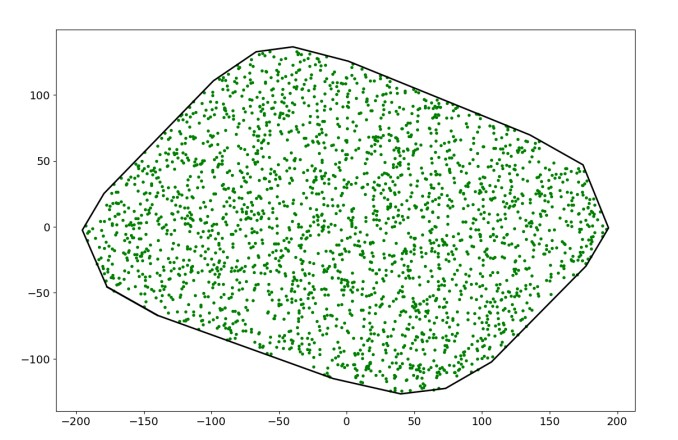
\includegraphics[width=350px]{./frame_polygon.jpg}
		\caption{Đa giác n điểm ngẫu nhiên có khung 16 cạnh ${\cal P}^\diamond$.}
		\label{frame_polygon}
	\end{center}
\end{figure} 	


Một vài hình ảnh kết quả chạy thuật toán Outer Convex Approximation với số điểm đầu vào bằng 100 được sinh ngẫu nhiên, và được đa giác 16 cạnh cắt thành tập các điểm nằm trong giới hạn kích thước nhỏ bao quanh mốc 150, với $\delta$ khác nhau (Hình \ref{outer_res_delta0}, \ref{outer_res_delta5}, \ref{outer_res_delta10}, \ref{outer_res_delta30}):
\begin{figure}[ht!]
	\begin{center}
		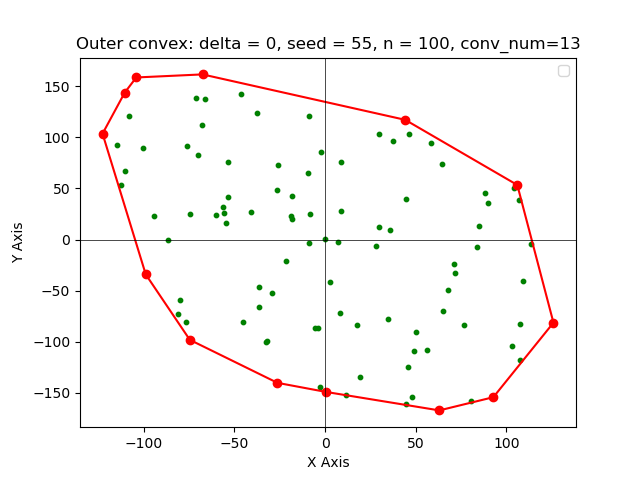
\includegraphics[width=350px]{./outer_res_delta0.png}
		\caption{Bao lồi kết quả khi chạy với $\delta$ = 0.}
		\label{outer_res_delta0}
	\end{center}
\end{figure} 	
\begin{figure}[ht!]
	\begin{center}
		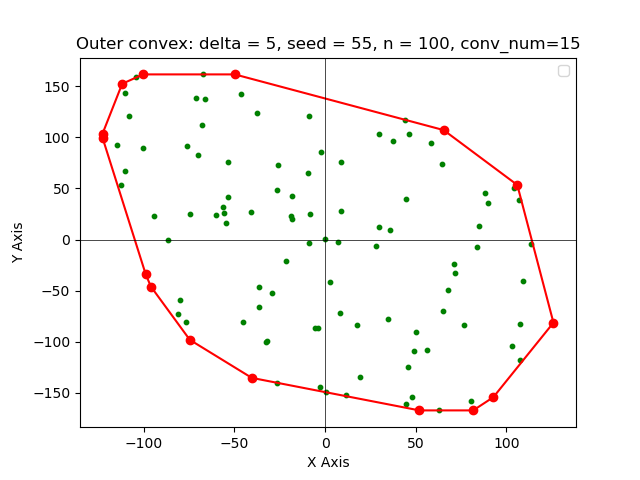
\includegraphics[width=350px]{./outer_res_delta5.png}
		\caption{Bao lồi kết quả khi chạy với $\delta$ = 5.}
		\label{outer_res_delta5}
	\end{center}
\end{figure} 	
\begin{figure}[ht!]
	\begin{center}
		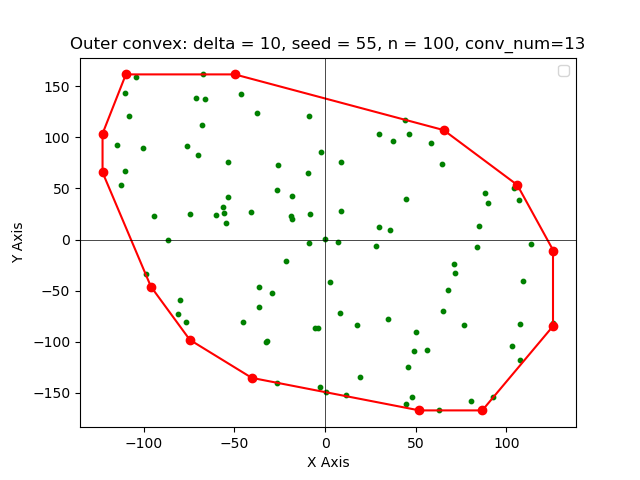
\includegraphics[width=350px]{./outer_res_delta10.png}
		\caption{Bao lồi kết quả khi chạy với $\delta$ = 10.}
		\label{outer_res_delta10}
	\end{center}
\end{figure} 	
\begin{figure}[ht!]
	\begin{center}
		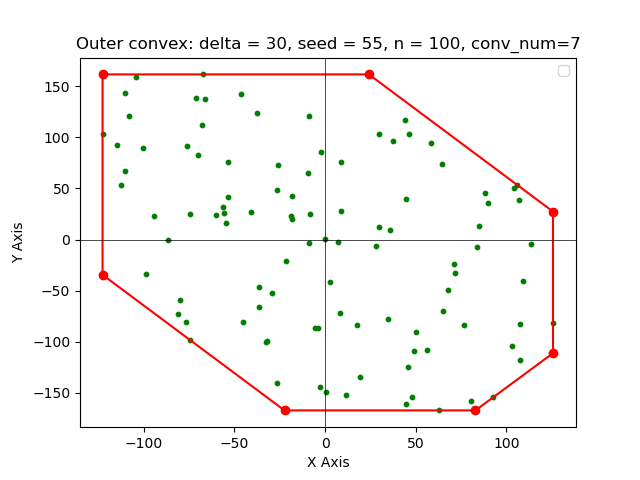
\includegraphics[width=350px]{./outer_res_delta30.png}
		\caption{Bao lồi kết quả khi chạy với $\delta$ = 30.}
		\label{outer_res_delta30}
	\end{center}
\end{figure} 	
\section{Inner convex approximation}\label{InnerConvexApproximation}

Cho $X$ thỏa mãn (\ref{ct2.1})--(\ref{ct2.2}) và $\delta \geq 0$, ở đây ta sẽ tìm một bao lồi xấp xỉ lồi trong ${\cal P}^{\rm inner}$  của $X$, tức là:
\begin{equation}\label{ct2.37}
	{\cal P}^{\rm inner} := \ conv X', \ \mbox{ với} X' \subset X,
\end{equation}
Sao cho:
\begin{equation}\label{ct2.38}
	\ dist_{\rm H}(\ conv X, {\cal P}^{\rm inner}) \leq \delta.
\end{equation}

Ta mô tả ${\cal P}^{\rm inner}$ bởi tập $E$ của các cạnh có hướng của nó $[p, p^+]$, trong đó $p^+$  là đỉnh kế tiếp ngược chiều kim đồng hồ của $p$, tức là:
\begin{equation}\label{ct2.39}
	E := \{[p, p^+] \mid p, p^+ \in X', \mbox{ $[p, p^+]$ là một cạnh của ${\cal P}^{\rm inner}$}\}.
\end{equation}


Ta bắt đầu quá trình tìm bao lồi xấp xỉ trong với tứ giác $\bar q_1 \bar q_2 \bar q_3 \bar q_4$, tức là:
\begin{equation}\label{ct2.40}
	\begin{array}{lcl}
		X' &:=& \{\bar q_1, \bar q_2, \bar q_3, \bar q_4\}, \\
		E &:=& \{[\bar q_1, \bar q_2], \, [\bar q_2, \bar q_3], \, [\bar q_3, \bar q_4], \, [\bar q_4, \bar q_1]\},
	\end{array}
\end{equation}
Trong đó $\bar q_1$, $\bar q_2$, $\bar q_3$, và $\bar q_4$ là độc nhất và được xác định bởi:
\begin{equation}\label{ct2.41}
	\begin{array}{lcl}
		x^1_{\rm min} &:=& \min \{x^1 \mid (x^1, x^2) \in X\}, \\
		x^1_{\rm max} &:=& \max \{x^1 \mid (x^1, x^2) \in X\}, \\
		x^2_{\rm min} &:=& \min \{x^2 \mid (x^1, x^2) \in X\}, \\
		x^2_{\rm max} &:=& \max \{x^2 \mid (x^1, x^2) \in X\}
	\end{array}
\end{equation}

\begin{equation}\label{ct2.42}
	\begin{array}{lcl}
		X^1_{\rm min} &:=& \{(x^1, x^2) \in X \mid x^1 = x^1_{\rm min}\}, \\
		X^1_{\rm max} &:=& \{(x^1, x^2) \in X \mid x^1 = x^1_{\rm max}\}, \\
		X^2_{\rm min} &:=& \{(x^1, x^2) \in X \mid x^2 = x^2_{\rm min}\}, \\
		X^2_{\rm max} &:=& \{(x^1, x^2) \in X \mid x^2 = x^2_{\rm max}\}
	\end{array}
\end{equation}
Và
\begin{equation}\label{ct2.43}
	\begin{array}{lcl}
		&& \bar q_1 = (\bar q_1^1, \bar q_1^2) \in X^1_{\rm max} \mbox{ thỏa mãn } \bar q_1^2 = \max\{x^2 \mid (x^1, x^2) \in X^1_{\rm max}\}, \\
		&& \bar q_2 = (\bar q_2^1, \bar q_2^2) \in X^2_{\rm max} \mbox{  thỏa mãn} \bar q_2^1 = \min\{x^1 \mid (x^1, x^2) \in X^2_{\rm max}\}, \\
		&& \bar q_3 = (\bar q_3^1, \bar q_3^2) \in X^1_{\rm min} \mbox{  thỏa mãn } \bar q_3^2 = \min\{x^2 \mid (x^1, x^2) \in X^1_{\rm min}\}, \\
		&& \bar q_4 = (\bar q_4^1, \bar q_4^2) \in X^2_{\rm min} \mbox{  thỏa mãn } \bar q_4^1 = \max\{x^1 \mid (x^1, x^2) \in X^2_{\rm min}\}.
	\end{array}
\end{equation}
Lưu ý rằng hai trong số bốn điểm $\bar q_1$, $\bar q_2$, $\bar q_3$, và $\bar q_4$ có thể trùng nhau, nhưng (\ref{ct2.2}) ngầm định rằng phải ít nhất ba trong số chúng khác nhau.

Trong các bước tiếp theo, đa giác ${\cal P}^{\rm inner}$ được xây dựng và cải thiện 
như sau.\\
Với cạnh bất kỳ $[p, p^+] \in E$ ($p \not= p^+$), ta xác định:
\begin{equation}\label{ct2.44}
	\begin{array}{lcl}
		\bar d_{[p, p^+]}^{\, T} &:=& \|p^+ - p\|^{-1} R \, (p^+ - p)^T, \\
		X_{[p, p^+]} &:=& \{x \in X \mid \bar d_{[p, p^+]}\, x^T > \bar d_{[p, p^+]}\, p^T \},
	\end{array}
\end{equation}
Với
\begin{equation*}%\label{rotationmatrix}
	R := \begin{pmatrix}
		0 & 1 \\
		-1 & 0
	\end{pmatrix}.
\end{equation*}

Nếu $X_{[p, p^+]} \not= \emptyset$ thì xác định:
\begin{equation}\label{ct2.45}
	\begin{array}{lcl}
		\beta_{[p, p^+]} &:=& \max \{\bar d_{[p, p^+]}\, x^T \mid x \in X_{[p, p^+]}\}, \\
		B_{[p, p^+]} &:=& \{x \in X_{[p, p^+]} \mid \bar d_{[p, p^+]}\, x^T = \beta_{[p, p^+]}\}.
	\end{array}
\end{equation}
Nếu:
\begin{equation}\label{dct2.46}
	\beta_{[p, p^+]} - \bar d_{[p, p^+]}\, p^T \leq \delta
\end{equation}
Thì ta không cần phải mở rộng ${\cal P}^{\rm inner }$ theo hướng $\bar d_{[p, p^+]}$ nữa.

Ngược lại, nếu:
\begin{equation}\label{ct2.47}
	\beta_{[p, p^+]} - \bar d_{[p, p^+]}\, p^T > \delta
\end{equation}
thì xác định điểm:
\begin{equation}\label{ct2.48}
	\hat p \in B_{[p, p^+]} \hbox{ thỏa mãn } \|\hat p - p\| = \max\{\|x - p\| \mid x \in B_{[p, p^+]}\},
\end{equation}
Và cập nhập $X'$ và $B$ bởi
\begin{equation}\label{ct2.49}
	\begin{array}{lcl}
		X' &:=& X' \cup \{\hat p\}, \\
		E &:=& E \cup \{[p, \hat p], \, [\hat p, p^+]\},
	\end{array}
\end{equation}
Và xác định: 
\begin{equation}\label{ct2.50}
	\begin{array}{lcl}
		X_{[p, \hat p]} &:=& \{x \in X_{[p, p^+]} \mid \bar d_{[p, \hat p]}\, x^T > \bar d_{[p, \hat p]}\, p^T \}, \\
		X_{[\hat p, p^+]} &:=& \{x \in X_{[p, p^+]} \mid \bar d_{[\hat p, p^+]}\, x^T > \bar d_{[\hat p, p^T]}\, {\hat p}^T \}.
	\end{array}
\end{equation}
Lưu ý rằng ta chỉ xem xét $x \in X_{[p, p^+]}$ trong định nghĩa này của $X_{[p, \hat p]}$ và $X_{[\hat p, p^+]}$, nhưng tất cả $x \in X$ đều được định nghĩa (\ref{ct2.44}) của $X_{[p, p^+]}$.

Quy trình tìm bao lồi được trình bày trong thuật toán sau, trong đó  $E_{\rm doubt}$ biểu thị tập hợp các cạnh cần được kiểm tra.

\begin{algorithm}\label{alg04}  \rm 
	\floatname{algorithm}{Thuật toán}
	\caption{}  \label{al-blduoi4}
	\emph{Input:} Tập hữu hạn $X \subset \R^2$ và tham số xấp xỉ $\delta \geq 0$. \\
	\emph{Output:} Đa giác lồi xấp xỉ trong ${\cal P}^{\rm inner}$ được mô tả bởi $X'$ và $E$.
	\begin{enumerate}
		\item\label{stepIalg04} 
		Tìm $X'$ và $E$ theo (\ref{ct2.40})--(\ref{ct2.43}).\\
		Với mọi ${[p, p^+]} \in E$ xác định $d_{[p, p^+]}$ và $X_{[p, p^+]}$ theo (\ref{ct2.44}).\\
		Cho $E_{\rm doubt} := E$.
		
		\item\label{stepIIalg04} 
		 Chọn một cạnh $[p, p^+] \in E_{\rm doubt}$. \\
		Nếu $X_{[p, p^+]} = \emptyset$, đặt
		$E_{\rm doubt} := E_{\rm doubt} \setminus \{[p, p^+]\}$
		và đi tới bước \ref{stepIIIalg04}.\\
		Tìm $\beta_{[p, p^+]}$ và $B_{[p, p^+]}$ theo (\ref{ct2.45}). \\
		Nếu (\ref{dct2.46}) đúng, đặt
		$E_{\rm doubt} := E_{\rm doubt} \setminus \{[p, p^+]\}$
		Và đi tới bước \ref{stepIIIalg04}.\\
		Trường hợp còn lại, lấy $\hat p$ định nghĩa theo (\ref{ct2.48}),
		 cập nhật $X'$ và $E$ theo (\ref{ct2.49}), và xác định $X_{[p, \hat p]}$ và $X_{[\hat p, p^+]}$ theo (\ref{ct2.50}), đặt
		\begin{equation*}%\label{newBdoubt3}
			E_{\rm doubt} := (E_{\rm doubt} \setminus \{[p, p^+])\}) \cup \{[p, \hat p], \, [\hat p, p^+]\}.
		\end{equation*}
		
		\item\label{stepIIIalg04} 
		Nếu $E_{\rm doubt} \ne \emptyset$  thì quay lại bước \ref{stepIIalg04}.
		
		\item
		Trả về $X'$, $E$ và kết thúc thuật toán.
	\end{enumerate}
\end{algorithm}


\medskip
Bảng \ref{table03} cho thấy một số kết quả thử nghiệm, trong đó:
\begin{itemize}
	\item $\#_{\rm Edges@ Alg.\, 2}$  là số cạnh trung bình của đa giác xấp xỉ lồi bao ngoài ${\cal P}^{\rm inner}$ được trả về bởi thuật toán \ref{al-blduoi4},
	\item $\#_{\rm Step\, II @ Alg.\, 2}$ là số lần thực hiện trung bình của bước II của thuật toán \ref{al-blduoi4}.
\end{itemize}

\begin{table}[ht]
	\begin{center}\renewcommand{\arraystretch}{1.2}\small
		\setlength\tabcolsep{0.3cm}
		\begin{tabular}{|c|c||c|c|c|c|c|c|c|c|c|c|c|c|c|}
			%\hline
			\hline
			\multicolumn {2}{|c||}{\footnotesize $\#X=n$}  &50& 500& 1000& 2500& 5000& 7500\\ 
			\hline		
			\hline
			{ $\delta = 70$}
			
			& $\#_{\rm Edges@ Alg.\, 3}$  &6 & 6 & 6 & 6 & 6 & 6\\
			
			& $\#_{\rm Step\, II @ Alg.\, 3}$&8 & 8 & 8 & 8 & 8 & 8  \\
			\hline
			{ $\delta = 10$}
			
			& $\#_{\rm Edges@ Alg.\, 3}$  &9 & 10 & 10 & 11 & 12 & 11 \\
			
			& $\#_{\rm Step\, II @ Alg.\, 3}$&14 & 16 & 16 & 18 & 20 & 18\\
			\hline
			{ $\delta = 1$}
			
			& $\#_{\rm Edges@ Alg.\,3}$  &12 & 19 & 22 & 23 & 26 & 22 \\
			
			& $\#_{\rm Step\, II @ Alg.\, 3}$&20 & 34 & 40 & 42 & 48 & 40  \\
			\hline
			{ $\delta = 0$}
			
			& $\#_{\rm Edges@ Alg.\, 3}$  &12 & 23 & 30 & 38 & 43 & 43 \\
			
			& $\#_{\rm Step\, II @ Alg.\, 3}$&20 & 42 & 56 & 72 & 82 & 82  \\
			\hline
		\end{tabular}
		\caption{Số cạnh trung bình của đa giác lồi xấp xỉ lồi trong ${\cal P}^{\rm inner}$ trả về bởi thuật toán \ref{al-blduoi4} và số lần thực hiện trung bình của bước \ref{stepIIalg04} khi $X$ gồm $n$ điểm ngẫu nhiên trong đa giác có khung $16$ cạnh ${\cal P}^\diamond$ và được hiển thị trong hình \ref{frame_polygon}.}
		\label{table03}
	\end{center}
\end{table} 	

	\bigskip\noindent
	{\bf LƯU Ý (Liên quan đến bảng \ref{table03}):}  $n$ điểm ngẫu nhiên được trình bày trong bảng \ref{table03} phải được tạo ra trong đa giác có khung $16$ cạnh ${\cal P}^\diamond$ và hiển thị trong hình \ref{frame_polygon}.
	
	\bigskip

\medskip
Bảng \ref{table04}  thể hiện một số kết quả thực nghiệm về thời gian chạy của thuật toán Outer Convex Approximation khi $X$ gồm $n$ điểm ngẫu nhiên được trình bày trong bảng \ref{table03} phải được tạo ra trong đa giác có khung $16$ cạnh ${\cal P}^\diamond$ hiển thị trong hình \ref{frame_polygon}, trong đó

$T_{\rm Alg.\, 2}$ là thời gian chạy trung bình của thuật toán \ref{al-blduoi4}.

\begin{table}[ht]
	\begin{center}\renewcommand{\arraystretch}{1.2}\small
		\setlength\tabcolsep{0.05cm}
		\begin{tabular}{|c|c||c|c|c|c|c|c|c|c|c|}
			%\hline
			\hline
			\multicolumn {2}{|c||}{\footnotesize $\#X=n$} &50& 500& 1000& 2500& 5000& 7500\\ 
			\hline		
			\hline
			{ $\delta = 70$}
			
			& $T_{\rm Alg.\, 2}$  &0.002035 & 0.01511 & 0.03 & 0.065514 & 0.145027 & 0.197571 \\
			
			& $T_{\rm Alg.\, 2}/n$&4.06981e-05 & 3.02205e-05 & 3e-05 & 2.62054e-05 & 2.90054e-05 & 2.63428e-05 \\
			\hline
			{ $\delta = 10$}
			
			& $T_{\rm Alg.\, 2}$  &0.005001 & 0.026086 & 0.047984 & 0.13192 & 0.283488 & 0.402505 \\
			
			& $T_{\rm Alg.\, 2}/n$&0.0001000214 & 5.21712e-05 & 4.79844e-05 & 5.27678e-05 & 5.66977e-05 & 5.36673e-05 \\
			\hline
			{ $\delta = 1$}
			
			& $T_{\rm Alg.\, 2}$  &0.005164 & 0.052596 & 0.127814 & 0.291402 & 0.645425 & 0.814138\\
			
			& $T_{\rm Alg.\, 2}/n$&0.0001032829 & 0.0001051922 & 0.0001278136 & 0.0001165608 & 0.000129085 & 0.0001085517\\
			\hline
			{ $\delta = 0$}
			
			& $T_{\rm Alg.\, 2}$  &0.006178 & 0.063702 & 0.158502 & 0.486671 & 1.094417 & 1.650608 \\
			
			& $T_{\rm Alg.\, 2}/n$&0.0001235676 & 0.0001274037 & 0.0001585019 & 0.0001946683 & 0.0002188833 & 0.000220081\\
			\hline
		\end{tabular}
		\caption{Thời gian chạy trung bình $T_{\rm Alg.\,2}$  thuật toán \ref{al-blduoi4} khi $X$ gồm $n$ điểm ngẫu nhiên được trình bày trong bảng \ref{table04} phải được tạo ra trong đa giác có khung $16$ cạnh  ${\cal P}^\diamond$ hiển thị trong hình \ref{frame_polygon}.}
		\label{table04}
	\end{center}
\end{table} 	


\chapter{Thực nghiệm và kết quả}

Chương này trình bày cách thức triển khai của đồ án: khởi tạo môi trường chạy, lấy tập dữ liệu DOTA, chuyển đổi thuật toán từ mã Python sang mã C++, thay thế thuật toán mới cho thuật toán cũ, cấu hình file config để thực hiện huấn luyện, một vài kết quả số.
\section{Khởi tạo môi trường chạy} 

Môi trường được sử dụng trong đồ án là Linux, bản phân phối Ubuntu 20.04.06 LTS, sử dụng 2 máy có thông số khác nhau để chạy. Một máy laptop với GTX 1650 4GB RAM và một máy pc RTX 3060 12GB RAM. CUDA Toolkit sử dụng phiên bản 11.6, cài đặt CUDNN.

Do code trong paper BeyoundBoundingBox đã không còn tương thích với phiên bản MMCV \cite{MMCV} hiện đại, em đã chuyển qua sử dụng thư viện MMROTATE, một thư viện mới được xây dựng vài tháng gần đây, có triển khai lại paper trên như là một bộ phát hiện mới, có tên là CFA. Thực hiện tải về các thư viện MMCV==1.7.1, MMDETECTION==2.28.2 và MMROTATE==0.3.4. Riêng 2 thư viện MMCV và MMROTATE \cite{MMRotate} thì clone git về và xây dựng thư viện từ nguồn (build from source) theo như tài liệu của OpenMmlab. Thư viện MMCV đóng vai trò cung cấp các phép toán hỗ trợ ở mức thấp (sử dụng code CUDA C++ để lập trình tính toán cho card đồ hoạ). Thư viện MMDETECTION \cite{MMDetection} là một bộ thư viện chủ đạo (ngoài ra còn có MMYolo) của phòng nghiên cứu OpenMmlab, cung cấp nền tảng để xây dựng tiếp một nhánh khác đó chính là thư viện MMROTATE. 

OpenMmlab là một dự án mã nguồn mở phục vụ cho nghiên cứu học thuật và ứng dụng công nghiệp, bao gồm nhiều chủ đề nghiên cứu trong lĩnh vực thị giác máy tính như: phân loại hình ảnh, phát hiện mục tiêu, phân đoạn mục tiêu, tạo hình ảnh siêu phân giải, và nhiều hơn nữa.

Từ khi được mở cửa vào năm 2018, OpenMmlab đã phát hành hơn 20 thư viện thuật toán, bao gồm hơn 250 cách triển khai thuật toán và 2000 mô hình được huấn luyện trước. OpenMmlab đã thu hút được hơn 60,000+ người theo dõi trên GitHub, với sự tham gia của hơn 1,300 nhà phát triển cộng đồng.

OpenMmlab cung cấp các thư viện chất lượng cao để giảm khó khăn trong việc tái cài đặt thuật toán, tạo ra chuỗi công cụ triển khai hiệu quả hướng đến nhiều backend và thiết bị khác nhau2. Dựa trên PyTorch, OpenMmlab phát triển MMEngine để cung cấp động cơ đào tạo và đánh giá phổ biến, và MMCV để cung cấp các toán tử mạng nơ-ron và biến đổi dữ liệu, phục vụ như một nền tảng cho toàn bộ dự án.

OpenMmlab đã phát hành hơn 30 thư viện thị giác, đã triển khai hơn 300 thuật toán, và chứa hơn 2000 mô hình được huấn luyện trước.

MMCV là một thư viện nền tảng cho nghiên cứu thị giác máy tính cung cấp các chức năng chính như sau:
\begin{itemize}
	\item xử lý ảnh/video
	\item trực quan hoá ảnh và nhãn của ảnh
	\item biến đổi ảnh
	\item các kiến trúc CNN khác nhau
	\item triển khai chất lượng cao của các phép tính CUDA phổ biến
\end{itemize}

MMDectection là một hộp công cụ phát hiện đối tượng chứa tập hợp các phương pháp phát hiện đối tượng phong phú, phân đoạn các thể hiện và phân đoạn toàn cảnh, cũng như  các thành phân liên quan và các mô đun. Dưới đây là toàn bộ khung của framework:
\begin{itemize}
	\item \textbf{api} cung cấp các APIs để hỗ trợ suy luận (inference)
	\item \textbf{structures} cung cấp các cấu trúc dữ liệu như bbox, mask, DetDataSample
	\item \textbf{datasets} hỗ trợ nhiều loai dataset khác nhau để phát hiện đối tượng, phân đoạn đối tượng, phân đoạn toàn cảnh
	\begin{itemize}
		\item \textbf{transforms} cung cấp nhiều phép biến đổi làm giàu dữ liệu
	   \item \textbf{samplers} định nghĩa các chiến lược mẫu nạp dữ liệu khác nhau
	\end{itemize}

	\item \textbf{models} là phần quan trọng nhất của bộ phát hiện, chứa các thành phần khác nhau của bộ phát hiện
	\begin{itemize}
	\item \textbf{detectors} \text{định nghĩa tất các các lớp mô hình phát hiện}
	\item \textbf{data\_preprocessors} \text{tiền xử lý dữ liệu đầu vào của mô hình}
	\item \textbf{backbones} \text{chứa nhiều mạng xương sống khác nhau} 
	\item \textbf{nexts} chứa \text{các thành phần cổ khác nhau của bộ phát hiện} 
	\item \textbf{dense\_heads} chứa phần đầu của bộ phát hiện thực hiện dự đoán dày đặc
	\item \textbf{roi\_heads} \text{chứa các phần đầu của bộ phát hiện dự đoán từ RoIs} 
	\item \textbf{seg\_heads} \text{chứa nhiều các head dành cho bài toán phân đoạn} 
	\item \textbf{losses} \text{ chứa các hàm loss khác nhau}
	\item \textbf{task\_modules}  cung cấp các module cho các tác vụ phát hiện cụ thể 
		 ví dụ: assigners, samplers, box coders và prior generators.
	\item \textbf{layers} \text{cung cấp một vài lớp mạng cơ bản}
	\end{itemize}
	\item \textbf{engine} là một phần của của các thành phần chạy
	\begin{itemize}
		\item \textbf{runner} cung cấp các thành phần mở rộng của MMengine's runner
		\item \textbf{schedulers} cung cấp bộ lập lich để điều chỉnh các siêu tham số tối ưu mạng
		\item \textbf{optimizers} cung cấp bộ tối ưu và lớp bao tối ưu
		\item \textbf{hooks} cung cấp các phần móc kết nối của bộ chạy
		
	\end{itemize}
	\item \textbf{evaluation} cung cấp các tham số khác nhau để đánh giá hiệu năng của mô hình
	\item \textbf{visualization} dùng để trực quan hoá các kết quả phát hiện
	
	
\end{itemize}

\begin{figure}[ht!]
	\begin{center}
		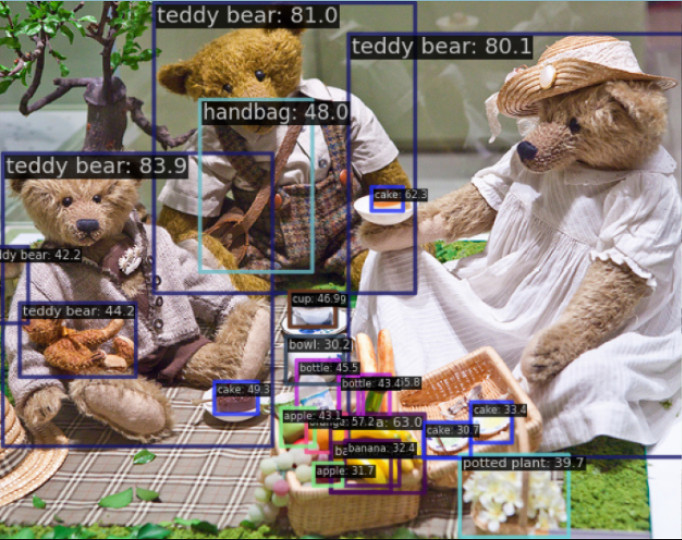
\includegraphics[width=445px]{./demo_mmrotate_result.jpg}
		\caption{Minh hoạ kết quả hình ảnh output của thư viện MMROTATE.}
		\label{demo_mmrotate_result}
	\end{center}
\end{figure} 

\section{Tập dữ liệu DOTA} 

Tập dữ liệu được sử dụng trong đồ án chính là tập dữ liệu DOTA v1.0. Tập dữ liệu DOTA được thu thập từ nền tảng Google Earth, GF-2 và vệ tinh JL-1 được cung cấp bởi Trung tâm Trung quốc nghiên cứu dữ liệu vệ tinh và ứng dụng, và các hình ảnh trên không được cung cấp bởi CycloMedia B.V. DOTA bao gồm các ảnh RGB và các ảnh mức xám. Tất cả các ảnh đều được lưu trữ dưới định dạng png. (\textit{bổ sung trích dẫn vào đây}). Tập dữ liệu DOTA có 3 phiên bản: v1.0, v1.5 và v2.0. Riêng tập dữ liệu v1.0 đã được chia sẵn các tập train, test, val.

Danh mục các đối tượng trong tập DOTA v1.0 bao gồm: \textit{plane, ship, storage tank, baseball diamond, tennis court, basketball court, ground track field, harbor, bridge, large vehicle, small vehicle, helicopter, roundabout, soccer ball field and swimming pool.}

Về định dạng nhãn, mỗi đối tượng được gán nhãn bởi một hộp bao có hướng (oriented bounding box - OBB), được ký hiệu là: $(x_1, y_1, x_2, y_2, x_3, y_3, x_4, y_4)$. Trong đó $(x_i, y_i)$ biểu thị đỉnh thứ i của OBB. Các đỉnh được sắp xếp theo chiều kim đồng hồ. Ảnh \ref{minh_hoa_hop_bao_dota} minh hoạ trực quan các nhãn. Điểm màu vàng đại diện cho điểm bắt đầu, có nghĩa là: a) góc trái của máy bay, b) góc trái trên cùng của một phương tiện to, c) trung tâm của một sân bóng chày.

Mỗi một thể hiện trong file nhãn có thêm một danh mục (category) và độ khó (difficult) biểu thi liệu thể hiện này có khó nhận diện hay không (1 là khó, 0 là không khó). Các nhãn của một ảnh được lưu trong một file text với cùng tên file. Mỗi dòng trong file đại diện cho một thể hiện. Ví dụ:

$x_1, y_1, x_2, y_2, x_3, y_3, x_4, y_4$, category, difficult 

$x_1, y_1, x_2, y_2, x_3, y_3, x_4, y_4$, category, difficult 

...

Sau khi download được tập dữ liệu DOTA về máy, thực hiện tiền xử lý dữ liệu. Ở đây có thể sử dụng tool split ảnh có sẵn trong source code Mmrotate. Sử dụng lệnh để chia ảnh ra với 8 process, kích thước ảnh 1024 pixels, overlaps 200. Sau khi chia ta có cây thư mục của tập dữ liệu như sau:\\
\\
\\
\\
\\
\\


\dirtree{%
	.1 DOTA.
	.2 trainval.
		.3 images.
			.4 P001.png.
			.4 P003.png.
			.4 ....
		.3 annfiles.
			.4 P001.txt.
			.4 P003.txt.
			.4 ....
	.2 test.
		.3 images.	
			.4 P001.png.
			.4 P003.png.
		.3 annfiles.
			.4 P001.txt.
			.4 P003.txt.
}

Với annfiles chứa các file annotation của từng ảnh, images là thư mục chứa các ảnh.
\begin{figure}[ht!]
	\begin{center}
		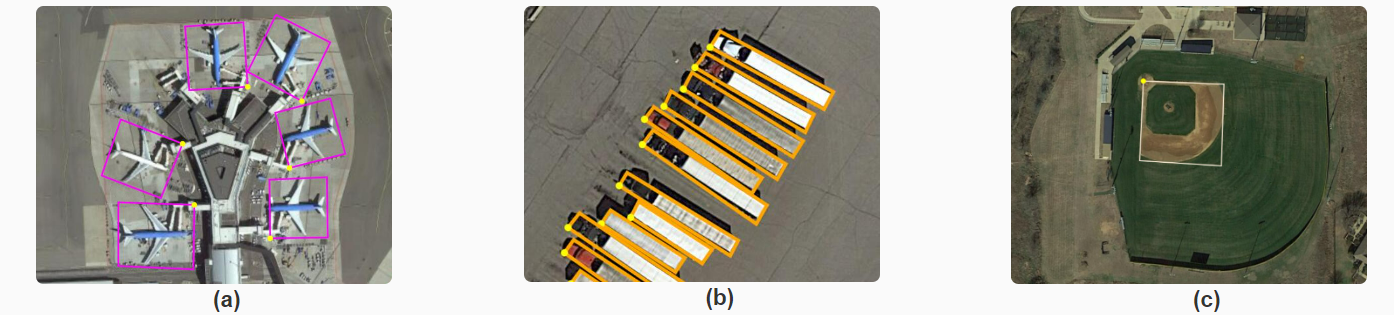
\includegraphics[width=445px]{./minh_hoa_hop_bao_dota.jpg}
		\caption{Minh hoạ nhãn hộp bao có hướng của tập dữ liệu DOTA.}
		\label{minh_hoa_hop_bao_dota}
	\end{center}
\end{figure} 
\subsection{Các bước thực hiện}
Tiếp theo thực hiện cài đặt miniconda, là một phiên bản thu gọn của Anaconda. Sau đó chạy các câu lệnh sau:


\begin{lstlisting}[language=bash, caption={Mô tả lệnh command line để tạo môi trường ảo}, label={lst:command-line}]

$ conda create -n mmrotate_v26_beta1 --no-default-packages \
 python==3.9 -y 
$ conda activate mmrotate_v26_beta1 
$ conda config --add channels conda-forge 
$ conda install pytorch==1.12.1 torchvision==0.13.1\ 
torchaudio==0.12.1 \
cudatoolkit=11.6 -c pytorch -c conda-forge 
$ cd mmcv
$ git checkout v1.7.1
$ pip install -r requirements/optional.txt 
$ MMCV_WITH_OPS=1 pip install -e . -v 
$ pip install mmdet==2.28.2 
$ cd ../mmrotate 
$ git checkout v0.3.4
$ pip install -v -e . 
$ conda install packaging 
$ conda install scipy 
$ conda install python-dateutil
$ pip install future tensorboard

\end{lstlisting}

Tiếp theo cần phải thay thế code thuật toán mới vào thuật toán Jarvis. Để thay thế được ta cần phải thay thế vào thư viện mmcv, tìm đến kernel convex\_iou\_kernel.cuh để thay thế 2 hàm Jarvis và Jarvis\_and\_index. Hai hàm hày có đầu vào là một mảng các Point tên là in\_poly đại diện cho số điểm cần tìm bao lồi, n\_poly đại diện cho số lượng phần tử trong mảng in\_poly. Đầu tiên thay thế bằng thuật toán Outer Convex Approximation thứ nhất. Thuật toán này có code Python như sau:

\begin{lstlisting}[language=Python, caption={Mô tả mã nguồn Python}, label={lst:python-code}]
# import cac thu vien can thiet
import numpy as np
import math
import matplotlib.pyplot as plt

np.random.seed(42)

# Khoi tao N_square
N_square = 10000

k = 16
count = 0
count1 = 0
count2 = 0
count3 = 0
count4 = 0


def outer_convex_approximation(X, delta):
# Rotation angle
alpha = -math.pi / 2

# Rotation Matrix
R = np.array([[math.cos(alpha), math.sin(alpha)], 
	 [-math.sin(alpha), math.cos(alpha)]])
#     print("Tap X: ", X)
# Step I: Determine D and P
D = [(1, 0), (0, 1), (-1, 0), (0, -1)]  # khoi tao D
       		 # theo cong thuc (7)
# cong thuc (8)
min_x = np.min((X[:, 0]))
max_x = np.max(X[:, 0])
min_y = np.min((X[:, 1]))
max_y = np.max(X[:, 1])

#  r1, r2, r3, r4 duoc dat theo
# cong thuc (10)
r1 = (max_x, max_y)
r2 = (min_x, max_y)
r3 = (min_x, min_y)
r4 = (max_x, min_y)

# Khoi tao P theo cong thuc (9)
P = np.array([r1, r2, r3, r4]) 

# STEP II: gan Pdoubt = P
Pdoubt = P[:]
Ptest = P[:]
global count, count4, count1, count2, count3
# Step III: lap den khi Pdoubt rong
# Dat bien count de xem so lan chay

# Neu so dinh Pdoubt > 0, tiep tuc lap
while Pdoubt.shape[0] > 0: 
count += 1
pdoubt = Pdoubt[0]  # lay gia tri pdoubt thuoc Pdoubt

# Xac dinh diem lien truoc va lien sau
# theo chieu kim dong ho cua pdoubt
pdoubt_index_idx = np.where(
      np.all(Ptest == pdoubt, axis=1))[0][0]
pdoubt_minus = Ptest[(pdoubt_index_idx - 1) % len(Ptest)]  # diem lien truoc
pdoubt_plus = Ptest[(pdoubt_index_idx + 1) % len(Ptest)]  # diem lien sau

# Xac dinh dp
dp = np.dot(R, ((pdoubt_minus - pdoubt_plus).T)) /
	 np.linalg.norm(pdoubt_minus - pdoubt_plus)

# xac dinh beta_dp
beta_dp = np.max(np.dot(dp, X.T))

# kiem tra cong thuc (16)

if beta_dp == np.dot(dp, pdoubt_plus):
count1 += 1
# Loai bo cac phan tu cua mang theo (17)
D.append(dp)  # Them dp vao danh sach D

P = np.delete(P, np.where(
	np.all(P == pdoubt, axis=1))[0], axis=0)
Pdoubt = np.delete(Pdoubt, np.where(
	np.all(Pdoubt == pdoubt, axis=1))[0], axis=0)
Ptest = np.delete(Ptest, np.where(
	np.all(Ptest == pdoubt, axis=1))[0], axis=0)


# Kiem tra (18) va (19)
elif np.dot(dp, pdoubt.T) - beta_dp > delta:
count2 += 1

# Khoi tao cong thuc (20)
lambda_p = (beta_dp - np.dot(dp, pdoubt_minus.T)) /
		 (np.dot(dp, pdoubt.T) 
		 - np.dot(dp, pdoubt_minus.T))  # lambda_p
p_hat_minus = (1 - lambda_p) * (pdoubt_minus.T) 
		+ lambda_p * (pdoubt.T)  # p^
p_hat_plus = (1 - lambda_p) * (pdoubt_plus.T)
		+ lambda_p * (pdoubt.T)  # p^+

D.append((dp[0], dp[1]))  # Them dp vao danh sach D
# tim chi so cua pdoubt trong mang Pdoubt
pdoubt_indexp = np.where(np.all(P == pdoubt, axis=1))[0][0]

# tim chi so cua pdoubt trong mang Pdoubt
pdoubt_index = np.where(np.all(Pdoubt == pdoubt, axis=1))[0][0]

# Xoa pdoubt khoi mang Pdoubt va
# them p_hat_minus va p_hat_plus
Pdoubt = np.delete(Pdoubt, pdoubt_index, axis=0)

if np.allclose(p_hat_plus, pdoubt) 
    and np.allclose(p_hat_minus, pdoubt):
count4 += 1
ptest_index = np.where(
		 np.all(Ptest == pdoubt, axis=1))[0][0]
Ptest = np.concatenate((Ptest[:ptest_index],
		 Ptest[ptest_index + 1:], [Ptest[ptest_index]]))

else:
# Xoa pdoubt khoi mang P
P = np.delete(P, pdoubt_indexp, axis=0)

# test voi Ptest
ptest_index = np.where(np.all(Ptest == pdoubt, axis=1))[0][0]
Ptest = np.delete(Ptest, ptest_index, axis=0)

if np.allclose(p_hat_plus, pdoubt_plus):
print("1")
else:
P = np.insert(P, pdoubt_indexp, p_hat_plus, axis=0)
Pdoubt = np.insert(Pdoubt, pdoubt_index, p_hat_plus, axis=0)
Ptest = np.insert(Ptest, ptest_index, p_hat_plus, axis=0)
if np.allclose(p_hat_minus, pdoubt_minus):
print("2")
else:
P = np.insert(P, pdoubt_indexp, p_hat_minus, axis=0)
Pdoubt = np.insert(Pdoubt, pdoubt_index, p_hat_minus, axis=0)
Ptest = np.insert(Ptest, ptest_index, p_hat_minus, axis=0)


# cac truong hop con lai
else:
count3 += 1
Pdoubt = np.delete(Pdoubt, np.where(np.all(Pdoubt == pdoubt, axis=1))[0][0],
axis=0)  # xoa pboubt khoi Pboubt

ptest_index = np.where(np.all(Ptest == pdoubt, axis=1))[0]
Ptest = np.concatenate((Ptest[:ptest_index[0]],
	 Ptest[ptest_index[0] + 1:], [Ptest[ptest_index[0]]]))

# Step V: Tra ve D va P
return D, P


# Kiem tra giai thuat voi du lieu
p1 = np.array([-130.658, -128])
p2 = np.array([-87.522, -128])
p3 = np.array([48.95, -104.547])
p4 = np.array([97.871, -89.647])
p5 = np.array([124.452, -69.508])
p6 = np.array([143.815, -35.205])
p7 = np.array([168, 62.629])
p8 = np.array([168, 96])
p9 = np.array([127.717, 128])
p10 = np.array([82.477, 128])
p11 = np.array([-61.85, 109.243])
p12 = np.array([-102.638, 98.195])
p13 = np.array([-124.269, 81.396])
p14 = np.array([-140.644, 46.529])
p15 = np.array([-168, -67.84])
p16 = np.array([-168, -99.849])

# Liet ke danh sach cac phan tu trong P
P = np.array([p1, p2, p3, p4, p5, p6, p7, p8, p9, p10,
   p11, p12, p13, p14, p15, p16, p1])


alpha = -math.pi / 2

# Ma tran xoay
R = np.array([[math.cos(alpha), math.sin(alpha)],
    [-math.sin(alpha), math.cos(alpha)]])

# Xoay mang P
po = np.dot(P, R)

# Determine min, max of p
# cong thuc (8)
x_min = np.nanmin(po[:, 0])
x_max = np.nanmax(po[:, 0])
y_min = np.nanmin(po[:, 1])
y_max = np.nanmax(po[:, 1])

xy_min = [x_min, y_min]
xy_max = [x_max, y_max]

# Khoi tao X
X = np.random.uniform(low=xy_min, high=xy_max,
       size=(N_square, 2))


def outside(points, a, b):
res = np.array([])
nx = b[1] - a[1]
ny = a[0] - b[0]
d = nx * a[0] + ny * a[1]
l = nx * points[:, 0] + ny * points[:, 1]
res = np.append(res, l - d >= 0)
return res


# Delete the points outside the polygon to creat a test set
for j in range(k):
X = np.delete(X, np.where(outside(X[:], po[j], po[j + 1])), 0)
X = X[0:50]

delta = 0.0
D, P = outer_convex_approximation(X, delta)
print("=====================tap D=====================")
for i in D:
print(i)
print("=====================tap P=====================")
for i in P:
print(i)
print("So dinh P: ", P.shape[0])

# Plotting
from scipy.spatial import ConvexHull

# Tao cac mang x, y tu tap P
x = P[:, 0]
y = P[:, 1]

# Tim bao loi cua tap diem
points = np.column_stack((x, y))
hull = ConvexHull(points)

# Lay cac diem tren bao loi
convex_points = points[hull.vertices]

# Them diem dau tien va diem cuoi cung
# vao thanh da giac hoan chinh
convex_points = np.vstack((convex_points, convex_points[0]))

# Plotting
fig, ax = plt.subplots(figsize=(8, 8))
ax.plot(X[:, 0], X[:, 1], 'r.')
ax.plot(P[:, 0], P[:, 1], 'r.')
ax.plot(convex_points[:, 0], convex_points[:, 1],
   'k-', linewidth=2)
ax.set_xlabel('X', fontsize=12)
ax.set_ylabel('Y', fontsize=12)
ax.set_title('Outer Convex Approximation', fontsize=14)
plt.grid(True)
plt.show()
\end{lstlisting}


Kết quả của thuật toán trên chạy được như sau:

=====================tap D=====================\\
(1, 0)\\
(0, 1)\\
(-1, 0)\\
(0, -1)\\
(0.7961489047057314, 0.6051007532104583)\\
(0.9616657625387172, 0.2742242898811617)\\
(0.9970047924756573, 0.07733979428839684)\\
(0.9997125319367726, 0.023976102447383348)\\
(0.9991870149267179, 0.04031512373582385)\\
(0.9992238689619551, 0.03939111189978383)\\
(0.9644107585317357, 0.2644085642112263)\\
(0.966079763964431, 0.2582438569616504)\\
(0.8253570386950088, 0.5646111570599768)\\
(0.8281780808160076, 0.5604650448118191)\\
(0.06376934956809235, 0.9979646637309673)\\
$[0.16708673 0.9859422]$\\
(-0.9549076761020365, 0.2969028967885088)\\
(-0.3704427977145033, 0.9288552813121382)\\
(-0.027620690279301655, 0.9996184759539485)\\
(-0.00775533544633372, 0.9999699269338628)\\
(-0.9248619391440728, 0.38030302854784814)\\
$[-0.86108908  0.50845413]$\\
(-0.9996753207961744, 0.025480443305911808)\\
(-0.9736272479423732, 0.22814465162295683)\\
(-0.7456221090230699, -0.6663690197900778)\\
(-0.9485403472713666, -0.3166562956871619)\\
(-0.9781544815182065, -0.2078793166379199)\\
(-0.9851213832260862, -0.17186000206773738)\\
(-0.9939783191936558, -0.10957691806651215)\\
(-0.9694661381128835, -0.2452252169995803)\\
(-0.2404163108063484, -0.9706698705009161)\\
(-0.41487577608285514, -0.9098780634896353)\\
(-0.6756181530719187, -0.7372517285430326)\\
(-0.1108120877182518, -0.993841376284728)\\
(-0.22747015261849787, -0.9737850531137338)\\
(0.6453245779421027, -0.7639084952426219)\\
(0.43292394969208786, -0.9014304486664528)\\
(0.19846709 -0.98010755)\\
(0.86030391 -0.50978151)\\
=====================tap P=====================\\
$\left[104.33701733 -84.23781101\right]$\\
$\left[100.49510361  13.21899328\right]$\\
$\left[92.95447702 41.42817061\right]$\\
$\left[ 25.06239458 141.74974297\right]$\\
$\left[-32.11772958 151.44000695\right]$\\
$\left[-111.3467922   150.82554052\right]$\\
$\left[-119.19653859  137.5316551 \right]$\\
$\left[-126.58633802  105.99503996\right]$\\
$\left[-119.95412846   45.83389818\right]$\\
$\left[ -81.45280839 -106.37608469\right]$\\
$\left[ -50.01887509 -135.18216969\right]$\\
$\left[  23.65812963 -152.39266133\right]$\\
$\left[  69.44520875 -143.12099702\right]$\\
So dinh P:  13\\


Thuật toán có mã Python như trên, cần phải chuyển đổi về mã CUDA C++ để thay thế thuật toán Jarvis ở trong thư viện MMCV. 

Mã CUDA C++ sẽ được thay thế vào hàm Jarvis của file cuda\_iou\_kernel.cuh. Trước tiên ta có vài hàm dùng chung như sau:


\begin{lstlisting}
#define MAXN_CUSTOM 99999
#define MAXN 100
#define NMAX 512
#define NMIN -999999

__device__ const double EPS = 1E-8;

__device__ inline int sig(double d)
 { return (d > EPS) - (d < -EPS); }

struct Point {
	double x, y;
	__device__ Point() {}
	__device__ Point(double x, double y) : x(x), y(y) {}
};
//====bat dau sua code tu day=====
// Ham tinh giai thua
__device__ inline double factorial(int n) {
	if (n == 0 || n == 1) {
		return 1;
	} else {
		return n * factorial(n - 1);
	}
}
// Ham tinh luy thua
__device__ inline double power(double base, int exponent) {
	double result = 1.0;
	for (int i = 0; i < exponent; ++i) {
		result *= base;
	}
	return result;
}
// Ham tinh sin theo phuong phap Taylor
__device__ inline double sin(double x) {
	int terms = 10;
	double result = 0.0;
	for (int n = 0; n < terms; ++n) {
		result += power(-1, n) * 
		power(x, 2 * n + 1) / factorial(2 * n + 1);
	}
	return result;
}
__device__ inline double sqrt(double x) {
	if (x < 0) {
		return -1;
	}
	
	double guess = x / 2;
	double previous_guess = 0;
	
	while (guess != previous_guess) {
		previous_guess = guess;
		guess = (guess + x / guess) / 2;
	}
	
	return guess;
}
// Ham tinh cos theo phuong phap Taylor
__device__ inline double cos(double x) {
	return sqrt(1 - sin(x) * sin(x));
}
//tinh max cua hai diem
__device__ inline double f_max(double x, double y) {
	if (x > y) {
		return x;
	}
	else {
		return y;
	}
}
__device__ inline double fabs(double x) {
	if (x >= 0) {
		return x;
	}
	else {
		return -x;
	}
}


//copy phan tu tu mang nay sang mang khac
__device__ inline void copy_points(
Point* src, Point* dst, int& n_src, int& n_dst) {
	// Sao chep tung phan tu cua mang
	for (int i = 0; i < n_src; i++) {
		if (src[i].x != NMIN && src[i].y != NMIN) {
			dst[i].x = src[i].x;
			dst[i].y = src[i].y;
		}
		
	}
	//thay doi lai so phan tu cua mang in_poly
	n_dst = n_src;
}

__device__ inline void find_all_point(
Point *P, int n, Point p, int result[]) {
	// khoi tao mang ket qua
	
	for (int i = 0; i < n; i++) {
		result[i] = NMIN;
	}
	
	//Khoi tao bien dem
	int count = 0;
	
	// Duyet qua mang P
	for (int i = 0; i < n; i++) {
		// Neu phan tu P[i] khop voi phan tu can tim
		if (P[i].x == p.x && P[i].y == p.y) {
			// Them chi so cua phan tu
			// P[i] vao mang ket qua
			result[count++] = i;
		}
	}
}

//chen Point vao Point* theo index
__device__ inline void insert_point_to_index(
			Point* P, int& n, int index, Point p) {
	// Kiem tra index hop le
	if (index < 0 || index > n) {
		return;
	}
	
	// Di chuyen cac phan tu sau vi tri 
	// can chen len 1 vi tri
	for (int i = n; i > index; i--) {
		P[i] = P[i - 1];
	}
	
	// Chen phan tu vao vi tri can chen
	P[index].x = p.x;
	P[index].y = p.y;
	
	// Cap nhat kich thuoc cua mang
	n++;
}

//Xoa Point trong mang theo index
__device__ inline void delete_point_by_index(
				Point* P, int& n, int index) {
	// Kiem tra index co hop le
	if (index < 0 || index >= n) {
		return;
	}
	
	// di chuyen cac phan tu sau phan tu
	// can xoa len mot vi tri
	for (int i = index; i < n - 1; i++) {
		P[i] = P[i + 1];
	}
	P[n - 1].x = NMIN;
	P[n - 1].y = NMIN;
	// Cap nhat kich thuoc cua mang
	n--;
}

//di chuyen Point xuong cuoi mang
__device__ inline void move_point_to_end(
				Point* P, int n, int index) {
	// Luu tru phan tu can di chuyen 
	Point temp = P[index];
	
	// DI chuyen cac phan tu len mot vi tri
	for (int i = index; i < n - 1; i++) {
		P[i] = P[i + 1];
	}
	
	// Dat cac phan tu can di chuyen vao vi tri cuoi cung
	P[n - 1] = temp;
}

//kiem tra allclose cua ca hai Point
__device__ inline bool allclose(
		const Point& p1, const Point& p2,
		 double rtol = 1e-5, double atol = 1e-8) {
	// tinh do lech tuong doi cua hai phan tu x
	double rel_diff_x = fabs(p1.x - p2.x)
	    / (atol + rtol * f_max(fabs(p1.x), fabs(p2.x)));
	
	//tinh do lech tuong doi cua hai phan tu y
	double rel_diff_y = fabs(p1.y - p2.y)
	    / (atol + rtol * f_max(fabs(p1.y), fabs(p2.y)));
	
	// kiem tra xem ca hai do lech tuong doi
	// deu nho hon hoac bang 1
	return rel_diff_x <= 1.0 && rel_diff_y <= 1.0;
}

//xoa mot Point trong mang khong dung index
__device__ inline void delete_point(
		Point* P, int& n, Point pdoubt) {
	// Tim chi so cua phan tu can xoa
	int index = -1;
	for (int i = 0; i < n; i++) {
		if (P[i].x == pdoubt.x && P[i].y == pdoubt.y) {
			index = i;
			break;
		}
	}
	
	// Neu tim thay phan tu can xoa
	if (index != -1) {
		// di chuyen cac phan tu con lai len tren
		for (int i = index + 1; i < n; i++) {
			P[i - 1] = P[i];
		}
		
		// Thay the phan tu cuoi cung nullptr
		P[n - 1].x = NMIN;
		P[n - 1].y = NMIN;
		//giam n di mot don vi
		n--;
	}
}

//tim index cua Point trong mang
__device__ inline int find_index(
			Point* P, int n, Point pdoubt) {
	// Duyet qua tat ca cac phan tu cua P
	for (int i = 0; i < n; i++) {
		// Neu phan tu thu i khop voi pdoubt
		if (P[i].x == pdoubt.x && P[i].y == pdoubt.y) {
			// Tra ve chi so cua phan tu thu i
			return i;
		}
	}
	
	// Phan tu pdoubt khong ton tai
	return -1;
}

//cong hai ma tran cung chieu voi nhau
__device__ inline void add_two_matrix(
		double A[1][2], double B[1][2],
		 int m, int n, double C[1][2]) {
	
	for (int i = 0; i < m; i++) {
		for (int j = 0; j < n; j++) {
			C[i][j] = 0;
		}
	}
	for (int i = 0; i < m; i++) {
		for (int j = 0; j < n; j++) {
			// Cong cac phan tu
			// tuong ung cua hai ma tran
			C[i][j] = A[i][j] + B[i][j];
		}
	}
}

//nhan ma tran hai chieu voi mot so double
__device__ inline void multiply_matrix_with_double(
		double matrix[1][2], int n, int m,
		double scalar, double result[1][2]) {
	
	// thuc hien lap
	for (int i = 0; i < n; i++) {
		for (int j = 0; j < m; j++) {
			result[i][j] = matrix[i][j] * scalar;
		}
	}
	
}

//xoa Point trong mang
__device__ inline void deletePoint(
		Point* arr, int& n, Point p) {
	// Tim vi tri cua phan tu can xoa
	int index = 0;
	for (int i = 0; i < n; i++) {
		if (arr[i].x == p.x && arr[i].y == p.y) {
			index = i;
			break;
		}
	}
	
	// Di chuyen cac phan tu sau vi tri can xoa len 1 vi tri
	for (int i = index + 1; i < n; i++) {
		arr[i - 1] = arr[i];
	}
	
	// Gan null cho phan tu can xoa
	arr[n - 1].x = NMIN;
	arr[n - 1].y = NMIN;
	//giam so phan tu cua mang di
	n--;
}

//chuyen ma tran 2x1 ve kieu Point
__device__ inline void convert_double_to_point(
			double matrix[1][2], Point& point) {
	// Gan gia tri cho diem
	point.x = matrix[0][0];
	point.y = matrix[0][1];
}

//tich vo huong cua ma tran va Point
__device__ inline double dot_product(
	double matrix[1][2], Point point) {
	// Khoi tao tich vo huong
	double dot_product = 0;
	dot_product += matrix[0][0] * point.x
	 + matrix[0][1] * point.y;
	return dot_product;
}

//Lay ra phan tu lon nhat trong ma tran
__device__ inline double get_max_value(
    double mul_dp_xtranspose[1][50], int rows, int n_poly) {
	// Khoi tao gia tri max
	double max_value = -DBL_MAX;
	int max_index = -1;
	
	// Lap qua cac phan tu cua mang
	for (int i = 0; i < rows; i++) {
		for (int j = 0; j < n_poly; j++) {
			// So sanh gia tri hien tai
			// voi gia tri max
			if (mul_dp_xtranspose[i][j] > max_value) 
			{
			max_value = mul_dp_xtranspose[i][j];
			}
		}
	}
	
	// Tra ve gia tri max
	return max_value;
}
__device__ inline void transpose_matrix(
double A[][2], int cols, int rows, double A_transpose[][50]) {
	
	// Duyet qua tat ca cac phan tu cua ma tran A
	for (int i = 0; i < rows; i++) {
		for (int j = 0; j < cols; j++) {
			// Thuc hien chuyen vi ma tran
			A_transpose[j][i] = A[i][j];
		}
	}
}

// Ma tran chuyen vi cua con tro double**,
// chuyen ma tran doc thanh ma tran ngang
__device__ inline void transpose_dp(
double matrix[2][1], double transposed_matrix[1][2]) {
	// Gan gia tri cho ma tran chuyen vi
	transposed_matrix[0][0] = matrix[0][0];
	transposed_matrix[0][1] = matrix[1][0];
}


//chuyen Point sang double**
__device__ inline void convert_point_to_matrix(
Point* points, int n, double X[][2]) {
	for (int i = 0; i < n; i++) {
		X[i][0] = points[i].x;
		X[i][1] = points[i].y;
	}
}

// chia ma tran cho mot so
__device__ inline void 
divide_matrix_by_double_and_return_new_matrix
(double matrix[2][1], double dp[2][1], 
int rows, int cols, double d) {
	
	for (int i = 0; i < rows; i++) {
		for (int j = 0; j < cols; j++) {
			dp[i][j] = matrix[i][j] / d;
		}
	}
}

//tinh chuan Euclid 
__device__ inline double norm_2(Point p) {
	// Tinh binh phuong cua tung phan tu trong ma tran
	double x2 = p.x * p.x;
	double y2 = p.y * p.y;
	return sqrt(x2 + y2);
}

//nhan hai ma tran voi nhau
__device__ inline void multiply_matrix(
double A[2][2], double B[2][1], 
double C[2][1], int m, int n, int p) {
	//Khoi tao ma tran ket qua
	for (int i = 0; i < m; i++) {
		for (int j = 0; j < p; j++) {
			C[i][j] = 0;
		}
	}
	
	// Nhan hai ma tran
	for (int i = 0; i < m; i++) {
		for (int j = 0; j < p; j++) {
			for (int k = 0; k < n; k++) {
				C[i][j] += A[i][k] * B[k][j];
			}
		}
	}
}

__device__ inline void multiply_matrix(
double A[1][2], double B[2][50],
 double C[1][50], int m, int n, int p) {
	//Khoi tao ma tran ket qua
	
	for (int i = 0; i < m; i++) {
		for (int j = 0; j < p; j++) {
			C[i][j] = 0;
		}
	}
	
	//  Nhan hai ma tran
	for (int i = 0; i < m; i++) {
		for (int j = 0; j < p; j++) {
			for (int k = 0; k < n; k++) {
				C[i][j] += A[i][k] * B[k][j];
			}
		}
	}
}
//tru hai diem cho nhau
__device__ inline void subtract_points(
Point p1, Point p2, Point& p3) {
	p3.x = p1.x - p2.x;
	p3.y = p1.y - p2.y;
}

__device__ inline void convert_point_to_matrix(
Point p, double matrix[2][1]) {
	matrix[0][0] = p.x;
	matrix[1][0] = p.y;
}
//chuyen Point sang ma tran cot
// chi danh cho ma tran kich thuoc 1x2
__device__ inline void 
convert_point_to_row_matrix
(Point p, double matrix[1][2]) {
	matrix[0][0] = p.x;
	matrix[0][1] = p.y;
}
//Tim chi so cua Point trong mang
__device__ inline int 
find_point_index
(Point* Ptest, Point pdoubt) {
	
	int index = -1;
	for (int i = 0; i < MAXN_CUSTOM; i++) {
		if (Ptest[i].x == pdoubt.x &&
		 Ptest[i].y == pdoubt.y) {
			index = i;
			break;
		}
	}
	if (index == -1) {
		return -1;
	}
	return index;
}


//====ket thuc them ham=====
\end{lstlisting}

Hàm Jarvis sẽ được thay thế thành code dưới:

\begin{lstlisting}
__device__ inline void Jarvis(Point* in_poly, int& n_poly) {
	
	
	
	//global
	double delta = 0.0;
	//Khoi tao mang xoay R
	double alpha = -M_PI / 2;
	double R[2][2];
	
	R[0][0] = cos(alpha);
	R[0][1] = sin(alpha);
	R[1][0] = -sin(alpha);
	R[1][1] = cos(alpha);
	
	Point D[MAXN_CUSTOM];
	for (int i = 0; i < MAXN_CUSTOM; i++) {
		D[i].x = NMIN;
		D[i].y = NMIN;
	}
	D[0] = Point(1.0, 0.0);
	D[1] = Point(0.0, 1.0);
	D[2] = Point(-1.0, 0.0);
	D[3] = Point(0.0, -1.0);
	int D_size = 4;
	
	
	// Khoi tao cac gia tri ban dau
	double min_x = DBL_MAX;
	double min_y = DBL_MAX;
	double max_x = -DBL_MAX;
	double max_y = -DBL_MAX;
	
	for (int i = 0; i < n_poly; i++) {
		// Cap nhat gia tri nho nhat
		if (in_poly[i].x < min_x) {
			min_x = in_poly[i].x;
		}
		// Cap nhat gia tri nho nhat
		if (in_poly[i].y < min_y) {
			min_y = in_poly[i].y;
		}
		
		// Cap nhat gia tri lon nhat
		if (in_poly[i].x > max_x) {
			max_x = in_poly[i].x;
		}
		
		// Cap nhat gia tri lon nhat
		if (in_poly[i].y > max_y) {
			max_y = in_poly[i].y;
		}
	}
	
	//Khoi tao P
	Point P[MAXN_CUSTOM];
	for (int i = 0; i < MAXN_CUSTOM; i++) {
		P[i].x = NMIN;
		P[i].y = NMIN;
	}
	P[0] = Point( max_x, max_y );
	P[1] = Point( min_x, max_y );
	P[2] = Point( min_x, min_y );
	P[3] = Point( max_x, min_y );
	
	int size_P = 4;
	
	
	//Khoi tao Pdoubt
	Point Pdoubt[MAXN_CUSTOM];
	for (int i = 0; i < MAXN_CUSTOM; i++) {
		Pdoubt[i].x = NMIN;
		Pdoubt[i].y = NMIN;
	}
	Pdoubt[0] = Point( max_x, max_y );
	Pdoubt[1] = Point( min_x, max_y );
	Pdoubt[2] = Point( min_x, min_y );
	Pdoubt[3] = Point( max_x, min_y );
	int size_Pdoubt = 4;
	
	//Khoi tao Ptest
	Point Ptest[MAXN_CUSTOM];
	for (int i = 0; i < MAXN_CUSTOM; i++) {
		Ptest[i].x = NMIN;
		Ptest[i].y = NMIN;
	}
	Ptest[0] = Point( max_x, max_y );
	Ptest[1] = Point( min_x, max_y );
	Ptest[2] = Point( min_x, min_y );
	Ptest[3] = Point( max_x, min_y );
	
	int size_Ptest = 4;
	
	int count = 0, count4 = 0, 
	count1 = 0, count2 = 0, count3 = 0;
	
	
	while (size_Pdoubt > 0) {
		count += 1;
		Point pdoubt = Pdoubt[0];
		int pdoubt_index_idx 
		= find_point_index(Ptest, pdoubt);
		int pdoubt_minus_index 
		= (pdoubt_index_idx + size_Ptest - 1)
		 % size_Ptest;
		// Lay chi so cua mang lien sau
		int pdoubt_plus_index 
		= (pdoubt_index_idx + 1) % size_Ptest;
		// Lay phan tu cua mang lien truoc
		Point pdoubt_minus
		 = Ptest[pdoubt_minus_index];
		// Lay phan tu cua mang lien sau
		Point pdoubt_plus
		 = Ptest[pdoubt_plus_index];
		
		Point result_sub_pminus_plus = { 0, 0 };
		subtract_points(pdoubt_minus, 
		pdoubt_plus, result_sub_pminus_plus);
		
		// Chuyen doi P thanh ma tran cot
		double transposed_matrix[2][1];
		convert_point_to_matrix(
		result_sub_pminus_plus, transposed_matrix);
		// Thuc hien nhan ma tran chuyen vi voi R
		double result_mul_matrix[2][1];
		multiply_matrix(
		R, transposed_matrix, 
		result_mul_matrix, 2, 2, 1);
		
		// Tinh chuan norm 2
		double norm_sub_pminus_pplus
		 = norm_2(result_sub_pminus_plus);
		
		// Tinh dp
		double dp[2][1];
		divide_matrix_by_double_and_return_new_matrix(
		result_mul_matrix, dp,
		2, 1, norm_sub_pminus_pplus);
		
		// Chuyen X ve ma tran
		double X[50][2];
		convert_point_to_matrix(in_poly, n_poly, X);
		
		double X_transpose[2][50];
		transpose_matrix(X, 2, n_poly, X_transpose);
		
		//dp_tranpose 1x2
		double dp_transpose[1][2];
		transpose_dp(dp, dp_transpose);
		
		double mul_dp_xtranspose[1][50];
		multiply_matrix(
		dp_transpose, X_transpose,
		 mul_dp_xtranspose, 1, 2, n_poly);
		
		//tinh Bdp
		double beta_dp = get_max_value(
		mul_dp_xtranspose, 1, n_poly);
		
		//kiem tra ket qua cua
		// tich vo huong
		if (beta_dp == dot_product(
		dp_transpose, pdoubt_plus)) {
		count1 += 1;
		Point dp_transpose_point = { 0,0 };
		convert_double_to_point(
		dp_transpose, dp_transpose_point);
		D[D_size] = dp_transpose_point;
		D_size++;
		deletePoint(P, size_P, pdoubt);
		deletePoint(Pdoubt, size_Pdoubt, pdoubt);
		deletePoint(Ptest, size_Ptest, pdoubt);
		}
		
		else if (dot_product(dp_transpose, pdoubt) 
		- beta_dp > delta) {
		count2++;
		double lambda_p = (beta_dp 
		- dot_product(dp_transpose, pdoubt_minus))
		/ (dot_product(dp_transpose, pdoubt)
		 - dot_product(dp_transpose, pdoubt_minus));
			
			
		double pdoubt_minus_convert_to_matrix[1][2];
		convert_point_to_row_matrix(
		pdoubt_minus, pdoubt_minus_convert_to_matrix);
			
		double pdoubt_convert_to_matrix[1][2];
		convert_point_to_row_matrix(
		pdoubt, pdoubt_convert_to_matrix);
			
		double A[1][2];
		multiply_matrix_with_double(
		pdoubt_minus_convert_to_matrix,
		 1, 2, (1 - lambda_p), A);
			
		double B[1][2];
		multiply_matrix_with_double(
		pdoubt_convert_to_matrix,
		 1, 2, lambda_p, B);
			
		double p_hat_minus[1][2];
		add_two_matrix(A, B, 1, 2, p_hat_minus);
			
		double pdoubt_plus_convert_to_matrix[1][2];
		convert_point_to_row_matrix(
		pdoubt_plus, pdoubt_plus_convert_to_matrix);
			
		double C[1][2];
		multiply_matrix_with_double(
		pdoubt_plus_convert_to_matrix,
		 1, 2, (1 - lambda_p), C);
			
		double p_hat_plus[1][2];
		add_two_matrix(C, B, 1,
		 2, p_hat_plus);
			
		Point dp_transpose_point = { 0,0 };;
		convert_double_to_point(
		dp_transpose, dp_transpose_point);
		D[D_size] = dp_transpose_point;
		D_size++;
			
		int pdoubt_indexp = find_index(
		P, size_P, pdoubt);
			
		int pdoubt_index = find_index(
		Pdoubt, size_Pdoubt, pdoubt);
			
		delete_point(Pdoubt,
		size_Pdoubt, pdoubt);
		Point p_hat_minus_point = { 0,0 };
		Point p_hat_plus_point = { 0,0 };
		convert_double_to_point(
		p_hat_minus, p_hat_minus_point);
		convert_double_to_point(
		p_hat_plus, p_hat_plus_point);
		if (allclose(pdoubt,
		 p_hat_minus_point) &&
		  allclose(pdoubt,
		   p_hat_plus_point)) {
			count4++;
			int ptest_index =
			 find_point_index(Ptest, pdoubt);
			move_point_to_end(Ptest,
			 size_Ptest, ptest_index);
		}
else {
	delete_point_by_index(P, size_P, pdoubt_indexp);
	int ptest_index = find_point_index(Ptest, pdoubt);
	delete_point_by_index(Ptest, size_Ptest, ptest_index);
	Point p_hat_plus_point(0, 0);
	convert_double_to_point(p_hat_plus, p_hat_plus_point);
	if (allclose(p_hat_plus_point, pdoubt_plus)) {
		//cout << "1" << endl;
	}
else {
	Point p_hat_plus_point = { 0,0 };
	convert_double_to_point(
	p_hat_plus, p_hat_plus_point);
	insert_point_to_index(
	P, size_P, pdoubt_indexp, p_hat_plus_point);
	insert_point_to_index(
	Pdoubt, size_Pdoubt,
	 pdoubt_index, p_hat_plus_point);
	insert_point_to_index(
	Ptest, size_Ptest,
		 ptest_index, p_hat_plus_point);
		}
		Point p_hat_minus_point = { 0,0 };
		convert_double_to_point(
		p_hat_minus, p_hat_minus_point);
		if (allclose(p_hat_minus_point, pdoubt_minus)) {
			//cout << "2" << endl;
		}
		else {
	Point p_hat_minus_point = { 0,0 };
	convert_double_to_point(p_hat_minus, p_hat_minus_point);
	
	insert_point_to_index(P, size_P,
	 pdoubt_indexp, p_hat_minus_point);
	insert_point_to_index(Pdoubt, size_Pdoubt,
	 pdoubt_index, p_hat_minus_point);
	insert_point_to_index(Ptest, size_Ptest,
	 ptest_index, p_hat_minus_point);
			
			}
			
		}
	}
	else {
	count3++;
	delete_point(Pdoubt, size_Pdoubt, pdoubt);
	int ptest_index[MAXN_CUSTOM];
	find_all_point(Ptest, size_Ptest, pdoubt, ptest_index);
	int first_index = ptest_index[0];
	move_point_to_end(Ptest, size_Ptest, first_index);
	}
	
}
copy_points(P, in_poly, size_P, n_poly);
\end{lstlisting}

Một hàm khác cần thay thế là Jarvis\_and\_index(). Hàm này tương tự hàm Jarvis, nhưng bảo toàn thứ tự của các điểm trong bao lồi khi chúng còn là một tập hợp các điểm. Ta thêm vào đoạn code này phần đầu của hàm Jarvis\_and\_index():


\begin{lstlisting}
	//global
int n_input = n_poly;
Point input_poly[20];
for (int i = 0; i < n_input; i++) {
	input_poly[i].x = in_poly[i].x;
	input_poly[i].y = in_poly[i].y;
}
\end{lstlisting}
Tiếp theo ta thêm đoạn code tương tự đoạn code Jarvis bên trên. Cuối cùng ta thêm đoạn code sau đây để lấy được chỉ số của các điểm nằm trên bao lồi trong tập điểm gốc:

\begin{lstlisting}
for (int i = 0; i < n_poly; i++) {
 for (int j = 0; j < n_input; j++) {
 	if (point_same(in_poly[i], input_poly[j])) {
		points_to_convex_ind[i] = j;
		break;
  }
 }
}
\end{lstlisting}

Tiếp theo ta có file code dùng để tuỳ chỉnh huấn luyện. File code này được viết bằng mã Python:
\begin{lstlisting}
# from mmcv import collect_env
# print(collect_env())

from mmcv import Config
from mmrotate.datasets.builder import ROTATED_DATASETS
from mmrotate.datasets.dota import DOTADataset


@ROTATED_DATASETS.register_module()
class CustomDotaDataset(DOTADataset):
"""SAR ship dataset for detection."""
CLASSES = ('plane', 'baseball-diamond', 
'bridge', 'ground-track-field',
'small-vehicle', 'large-vehicle',
 'ship', 'tennis-court',
'basketball-court', 'storage-tank'
, 'soccer-ball-field',
'roundabout', 'harbor',
 'swimming-pool', 'helicopter')
cfg = Config.fromfile('./configs/
cfa/cfa_r50_fpn_40e_dota_oc.py')
from mmdet.apis import set_random_seed

cfg.dataset_type = 'CustomDotaDataset'
cfg.data_root = 'data/split_ss_dota/'

cfg.data.test.type = 'CustomDotaDataset'
cfg.data.test.data_root = 'data/split_ss_dota/'
cfg.data.test.ann_file = 'test/annfiles/'
cfg.data.test.img_prefix = 'test/images/'

cfg.data.train.type = 'CustomDotaDataset'
cfg.data.train.data_root = 'data/split_ss_dota/'
cfg.data.train.ann_file = 'trainval/annfiles/'
cfg.data.train.img_prefix = 'trainval/images/'

cfg.data.val.type = 'CustomDotaDataset'
cfg.data.val.data_root = 'data/split_ss_dota/'
cfg.data.val.ann_file = 'trainval/annfiles/'
cfg.data.val.img_prefix = 'trainval/images/'

cfg.work_dir = './results'
cfg.log_config.interval = 50

cfg.evaluation.interval = 5
cfg.checkpoint_config.interval = 1

# Set seed thus the results are more reproducible
cfg.seed = 0
set_random_seed(0, deterministic=False)
cfg.gpu_ids = range(1)
cfg.device='cuda'

import os.path as osp
import os
import mmcv
from mmdet.datasets import build_dataset
from mmdet.models import build_detector
from mmdet.apis import train_detector

import torch
torch.cuda.empty_cache()

# Build dataset
datasets = [build_dataset(cfg.data.train)]

# Build the detector
model = build_detector(
cfg.model, train_cfg=cfg.get('train_cfg'),
 test_cfg=cfg.get('test_cfg'))
# Add an attribute for visualization convenience
model.CLASSES = datasets[0].CLASSES
mmcv.mkdir_or_exist(osp.abspath(cfg.work_dir))
train_detector(model, datasets,
 cfg, distributed=False, validate=True)


\end{lstlisting}




\textbf{Đây là các hàm hỗ trợ cho Inner Convex Appoximation:}
\begin{lstlisting}
	
	struct Edge {
		Point first_point;
		Point second_point;
	};
	__device__ inline int findMinPointIndex(
	const Point points[], int n) {
	if (n <= 0) {
		return -1;
	}
	
	int minIndex = 0;
	
	for (int i = 1; i < n; ++i) {
		if (points[i].y < points[minIndex].y) {
			minIndex = i;
		}
		else if (points[i].y == points[minIndex].y &&
		 points[i].x < points[minIndex].x) {
			minIndex = i;
		}
	}
	
		return minIndex;
	}
	
__device__ inline void moveMinPointsToFront(
	Point points[], int n) {
	int minIndex = findMinPointIndex(points, n);
	Point points_premitive[20];
	for (int i = 0; i < n; i++) {
		points_premitive[i] = points[i];
	}
	if (minIndex != -1) {
		Point temp[20];
		int tempIndex = 0;

		for (int i = minIndex; i < n; ++i) {
			temp[tempIndex++] = points[i];
		}
		
		for (int i = 0; i < minIndex; ++i) {
			points[i + n - minIndex] 
			= points_premitive[i];
		}
		
		for (int i = 0; i < tempIndex; ++i) {
			points[i] = temp[i];
		}
	}
}
__device__ inline void reversePoints(
		Point* points, int size) {
	int start = 0;
	int end = size - 1;
	
	while (start < end) {
		Point temp = points[start];
		points[start] = points[end];
		points[end] = temp;
		
		++start;
		--end;
	}
}
__device__ inline void copy_points(
Point* src, Point* dst, int& n_src,
 int& n_dst) {
for (int i = 0; i < n_src; i++) {
	dst[i].x = src[i].x;
		dst[i].y = src[i].y;
		
	}
	n_dst = n_src;
}
__device__ inline bool pointExists(
const Point* uniquePoints,
 int size, const Point& p) {
	for (int i = 0; i < size; ++i) {
		if (uniquePoints[i].x == p.x && 
		uniquePoints[i].y == p.y) {
			return true;
		}
	}
	return false;
}

__device__ inline void uniquePoints(
const Edge* edges, int size,
 Point* uniquePoints, int& uniqueSize) {
	for (int i = 0; i < size; ++i) {
			if (!pointExists(uniquePoints,
	 uniqueSize, edges[i].first_point)) {
	 	uniquePoints[uniqueSize]
	 	 = edges[i].first_point;
				++uniqueSize;
			}
			
	if (!pointExists(uniquePoints, 
	uniqueSize, edges[i].second_point)) {
		uniquePoints[uniqueSize]
		 = edges[i].second_point;
		++uniqueSize;
	}
		}
	}
	
	//chen 1 canh vao phan tu
	__device__ inline void insert_edge(
	Edge* edges, int& n, 
	const Edge& edge, int index) {
		
		if (index == -1) {
			index = n;
		}
		for (int i = n - 1; i >= index; i--) {
			edges[i + 1] = edges[i];
		}
		
		edges[index] = edge;
		n++;
	}
	
	//xoa canh theo chi so
	__device__ inline void erase_edge(
	Edge* edges, int& n, int index) {
		if (index < 0 || index >= n) {
			return;
		}
		
		for (int i = index + 1; i < n; i++) {
			edges[i - 1] = edges[i];
		}
		
		n--;
	}
	
	//tim chi so cua 1 canh trong mang
	__device__ inline int find_edge_index(
	Edge* edges, int n, Edge& edge) {
		int index = -1;
		for (int i = 0; i < n; i++) {
			if (
	edges[i].first_point.x == edge.first_point.x &&
	edges[i].first_point.y == edge.first_point.y &&
	edges[i].second_point.x == edge.second_point.x &&
	edges[i].second_point.y == edge.second_point.y
	) {
				index = i;
				break;
			}
		}
		return index;
	}
	
__device__ inline double f_max(double x, double y) {
	if (x > y) {
		return x;
	}
	else {
		return y;
	}
}
	
__device__ inline void divide_colmatrix_by_double(
double matrix[2][1], double d) {
	
	for (int i = 0; i < 2; i++) {
		for (int j = 0; j < 1; j++) {
			matrix[i][j] = matrix[i][j] / d;
		}
	}
}

__device__ inline void multiply_R_matrix(
double R[2][2], double B[2][1], 
double C[2][1], int m = 2, int n = 2,
 int p = 1) {
		
for (int i = 0; i < m; i++) {
	for (int j = 0; j < p; j++) {
		C[i][j] = 0;
	}
}

for (int i = 0; i < m; i++) {
	for (int j = 0; j < p; j++) {
		for (int k = 0; k < n; k++) {
			C[i][j] += R[i][k] * B[k][j];
		}
	}
		}
	}
	
__device__ inline bool allclose(
const Point& p1, const Point& p2, 
double rtol = 1e-5, double atol = 1e-8) {
	double rel_diff_x = fabs(p1.x - p2.x) / 
	(atol + rtol * f_max(fabs(p1.x), fabs(p2.x)));
	
	double rel_diff_y = fabs(p1.y - p2.y) / 
	(atol + rtol * f_max(fabs(p1.y), fabs(p2.y)));
	
	return rel_diff_x <= 1.0 && rel_diff_y <= 1.0;
}

__device__ inline double findMaxValue(
double arr[], int size) {
		if (size <= 0) {
			return 0.0; 
		}
		
		double maxVal = arr[0];
		for (int i = 1; i < size; ++i) {
			if (arr[i] > maxVal) {
				maxVal = arr[i];
			}
		}
		
		return maxVal;
	}
	__device__ inline void delete_edges(
	Edge* edges, int& n, Edge edoubt) {
		int count = 0;
		
		for (int i = 0; i < n; i++) {
			if (
	(edges[i].first_point.x == edoubt.first_point.x &&
	edges[i].first_point.y == edoubt.first_point.y &&
	edges[i].second_point.x == edoubt.second_point.x &&
	edges[i].second_point.y == edoubt.second_point.y) ||
	(edges[i].first_point.x == edoubt.second_point.x &&
	edges[i].first_point.y == edoubt.second_point.y &&
	edges[i].second_point.x == edoubt.first_point.x &&
	edges[i].second_point.y == edoubt.first_point.y)
			) {
				count++;
			}
			else {
				edges[i - count] = edges[i];
			}
		}
		n -= count;
	}
	
__device__ inline void convert_point_to_colmatrix(
Point p, double matrix[2][1]) {
	matrix[0][0] = p.x;
	matrix[1][0] = p.y;
}
	
__device__ inline void transpose_to_colmatrix(
double matrix[1][2], double transposed_matrix[2][1]) {
	transposed_matrix[0][0] = matrix[0][0];
	transposed_matrix[1][0] = matrix[0][1];
}

__device__ inline void transpose_to_rowmatrix(
double matrix[2][1], double transposed_matrix[1][2]) {
	transposed_matrix[0][0] = matrix[0][0];
	transposed_matrix[0][1] = matrix[1][0];
}
	
__device__ inline double dot_product(
double matrix1[1][2], double matrix2[2][1]) {
double dot_product = 0;
dot_product += matrix1[0][0] * matrix2[0][0] +
 matrix1[0][1] * matrix2[1][0];
return dot_product;
}
	
__device__ inline void convert_many_points_to_matrix(
Point* points, int n, double X[][2]) {
	for (int i = 0; i < n; i++) {
		X[i][0] = points[i].x;
		X[i][1] = points[i].y;
	}
}
	
__device__ inline void 
divide_matrix_by_double_and_return_new_matrix(
double matrix[2][1], double dp[2][1], 
int rows, int cols, double d) {
	
	for (int i = 0; i < rows; i++) {
		for (int j = 0; j < cols; j++) {
			dp[i][j] = matrix[i][j] / d;
		}
	}
}
	
__device__ inline double norm_2(Point p) {
	double x2 = p.x * p.x;
	double y2 = p.y * p.y;
	
	return sqrt(x2 + y2);
}
	
__device__ inline double norm_2(Point p1, Point p2) {
	Point tmp = { 0, 0 };
	tmp.x = p1.x - p2.x;
	tmp.y = p1.y - p2.y;
	double x2 = tmp.x * tmp.x;
	double y2 = tmp.y * tmp.y;
	
	return sqrt(x2 + y2);
}
	
	
__device__ inline void
 convert_point_to_rowmatrix(
 Point p, double matrix[1][2]) {
	matrix[0][0] = p.x;
	matrix[0][1] = p.y;
}

__device__ inline void
 subtract_points(
 Point p1, Point p2, Point& p3) {
	p3.x = p1.x - p2.x;
	p3.y = p1.y - p2.y;
}
	
__device__ inline double
 find_max_x(Point X[], int n) {
	double max_x = X[0].x;
	
	for (int i = 1; i < n; i++) {
		if (X[i].x > max_x) {
			max_x = X[i].x;
		}
	}
	
	return max_x;
}
	
__device__ inline double
 find_min_x(Point X[], int n) {
	double min_x = X[0].x;
	for (int i = 1; i < n; i++) {
		if (X[i].x < min_x) {
			min_x = X[i].x;
		}
	}
	
	return min_x;
}
	
__device__ inline 
double find_max_y(Point X[], int n) {
	double max_y = X[0].y;
	for (int i = 1; i < n; i++) {
		if (X[i].y > max_y) {
			max_y = X[i].y;
		}
	}
	
	return max_y;
}
	
__device__ inline double
 find_min_y(Point X[], int n) {
	double min_y = X[0].y;
	for (int i = 1; i < n; i++) {
		if (X[i].y < min_y) {
			min_y = X[i].y;
		}
	}
	return min_y;
}
	
__device__ inline void find_points_by_x(
Point* X, int& n, double min_x,
 Point points[], int& size_point) {
	int count = 0;
	for (int i = 0; i < n; i++) {
		if (X[i].x == min_x) {
			points[count].x = X[i].x;
			points[count].y = X[i].y;
			count++;
		}
	}
	size_point = count;
}
	
__device__ inline void find_points_by_y(
Point* X, int n, double min_y,
 Point points[], int& size_point) {
	
	int count = 0;
	for (int i = 0; i < n; i++) {
		if (X[i].y == min_y) {
			points[count].x = X[i].x;
			points[count].y = X[i].y;
			count++;
		}
	}
	size_point = count;
}
\end{lstlisting}	
\textbf{Ta có hai hàm thay mới tương tự dành cho thuật toán Inner Convex Approximation:}

\begin{lstlisting}
__device__ inline void Jarvis(Point* in_poly, int& n_poly) {
	
	//global
	double delta = 0.0;
	double alpha = PI / 2;
	double R[2][2];
	
	R[0][0] = cos(alpha);
	R[0][1] = sin(alpha);
	R[1][0] = -sin(alpha);
	R[1][1] = cos(alpha);
	double min_x = in_poly[0].x;
	double max_x = in_poly[0].x;
	double min_y = in_poly[0].y;
	double max_y = in_poly[0].y;
	
	for (int i = 1; i < n_poly; i++) {
		if (in_poly[i].x < min_x) {
			min_x = in_poly[i].x;
		}
		
		if (in_poly[i].y < min_y) {
			min_y = in_poly[i].y;
		}
		if (in_poly[i].x > max_x) {
			max_x = in_poly[i].x;
		}
		
		if (in_poly[i].y > max_y) {
			max_y = in_poly[i].y;
		}
	}
	Point min_X[100];
	Point max_X[100];
	Point min_Y[100];
	Point max_Y[100];
	int size_min_X = 0;
	int size_max_X = 0;
	int size_min_Y = 0;
	int size_max_Y = 0;
	
	//tim cac diem co hoanh do nho nhat
find_points_by_x(in_poly, n_poly, min_x, min_X, size_min_X);
//tim cac diem co hoanh do lon nhat
find_points_by_x(in_poly, n_poly, max_x, max_X, size_max_X);
//tim cac diem co tung do nho nhat
find_points_by_y(in_poly, n_poly, min_y, min_Y, size_min_Y);
//tim cac diem co tung do lon nhat
find_points_by_y(in_poly, n_poly, max_y, max_Y, size_max_Y);

double q12 = find_max_y(max_X, size_max_X);
double q21 = find_min_x(max_Y, size_max_Y);
double q32 = find_min_y(min_X, size_min_X);
double q41 = find_max_x(min_Y, size_min_Y);

Point q1 = { max_x, q12 };
Point q2 = { q21, max_y };
Point q3 = { min_x, q32 };
Point q4 = { q41, min_y };

Point Xcomma[100];
Xcomma[0] = q1;
Xcomma[1] = q2;
Xcomma[2] = q3;
Xcomma[3] = q4;
int size_X_comma = 4;

Edge edge0 = { q1, q2 };
Edge edge1 = { q2, q3 };
Edge edge2 = { q3, q4 };
Edge edge3 = { q4, q1 };
//khoi tao E_test
Edge E_test[100];
E_test[0] = edge0;
E_test[1] = edge1;
E_test[2] = edge2;
E_test[3] = edge3;
int size_E_test = 4;

//khoi tao Edoubt
Edge Edoubt[100];
for (int i = 0; i < size_E_test; i++) {
	Edoubt[i] = E_test[i];
}
int size_Edoubt = size_E_test;

while (size_Edoubt > 0) {
Edge edoubt = Edoubt[0];
Point p = edoubt.first_point;
Point p_plus = edoubt.second_point;

//tinh dpp_plus theo cong thuc (44)
Point result_sub_pplus_p = { 0, 0 };
subtract_points(p_plus, p, result_sub_pplus_p);
double transposed_matrix[2][1];
convert_point_to_colmatrix(result_sub_pplus_p,
transposed_matrix);
double result_mul_matrix[2][1];
multiply_R_matrix(R, transposed_matrix, result_mul_matrix);
double norm_sub_pplus_p = norm_2(result_sub_pplus_p);
double dpp_plus[2][1];
divide_matrix_by_double_and_return_new_matrix(
result_mul_matrix, dpp_plus, 2, 1, norm_sub_pplus_p);
double X[100][2];
convert_many_points_to_matrix(in_poly, n_poly, X);
	
Point Xp_pplus[100];
int size_Xpp_plus = 0;
double dpp_plus_T[1][2];
transpose_to_rowmatrix(dpp_plus, dpp_plus_T);
double p_T[2][1];
convert_point_to_colmatrix(p, p_T);
double dpp_plus_mul_p_T = dot_product(dpp_plus_T, p_T);
for (int i = 0; i < n_poly; i++) {
double item_X_T[2][1];
item_X_T[0][0] = X[i][0];
item_X_T[1][0] = X[i][1];

double tmp = dot_product(dpp_plus_T, item_X_T);
if (tmp > dpp_plus_mul_p_T) {
Xp_pplus[size_Xpp_plus].x = X[i][0];
Xp_pplus[size_Xpp_plus].y = X[i][1];
size_Xpp_plus++;
}
}
if (size_Xpp_plus != 0) {
double X_p_pplus0[1][2];
X_p_pplus0[0][0] = Xp_pplus[0].x;
X_p_pplus0[0][1] = Xp_pplus[0].y;
double X_p_pplus0_T[2][1];
transpose_to_colmatrix(X_p_pplus0, X_p_pplus0_T);
double beta_p_pplus = dot_product(dpp_plus_T, X_p_pplus0_T);
for (int i = 0; i < size_Xpp_plus; i++) {
double item_X_p_pplus[1][2];
item_X_p_pplus[0][0] = Xp_pplus[i].x;
item_X_p_pplus[0][1] = Xp_pplus[i].y;
double item_X_p_pplus_T[2][1];
transpose_to_colmatrix(item_X_p_pplus, item_X_p_pplus_T);
double tmp = dot_product(dpp_plus_T, item_X_p_pplus_T);
if (tmp > beta_p_pplus) {
	beta_p_pplus = tmp;
}
}

Point Bpp_plus[100];
int size_Bpp_plus = 0;
for (int i = 0; i < size_Xpp_plus; i++) {
double item_Xpp_plus[1][2];
item_Xpp_plus[0][0] = Xp_pplus[i].x;
item_Xpp_plus[0][1] = Xp_pplus[i].y;
double item_Xpp_plus_T[2][1];
transpose_to_colmatrix(item_Xpp_plus, item_Xpp_plus_T);
if (dot_product(dpp_plus_T, item_Xpp_plus_T) == beta_p_pplus) {
Bpp_plus[size_Bpp_plus].x = Xp_pplus[i].x;
Bpp_plus[size_Bpp_plus].y = Xp_pplus[i].y;
size_Bpp_plus++;
}
}
if (beta_p_pplus - dot_product(dpp_plus_T, p_T) <= delta) {
	delete_edges(Edoubt, size_Edoubt, edoubt);
}
else {
Point p_hat[100];
int size_p_hat = 0;
Point p_hat_calc[100];
int size_p_hat_calc = 0;
for (int i = 0; i < size_Bpp_plus; i++) {
	p_hat_calc[size_p_hat_calc].x = Bpp_plus[i].x;
	p_hat_calc[size_p_hat_calc].y = Bpp_plus[i].y;
	size_p_hat_calc++;
}
Point X_calc[100];
int size_X_calc = 0;
for (int i = 0; i < size_Bpp_plus; i++) {
X_calc[size_X_calc].x = Bpp_plus[i].x;
X_calc[size_X_calc].y = Bpp_plus[i].y;
size_X_calc++;
}
Point p_hat_calc_sub_p = { 0, 0 };
subtract_points(p_hat_calc[0], p, p_hat_calc_sub_p);
//mang nay dung de tim max cua norm(x_calc - p)
double arr_norm_xcalc_p[100];

int size_arr_norm_xcalc_p = 0;
for (int i = 0; i < size_Bpp_plus; i++) {
Point x_calc_sub_p = { 0, 0 };
subtract_points(X_calc[i], p, x_calc_sub_p);
double res_norm = norm_2(x_calc_sub_p);
arr_norm_xcalc_p[size_arr_norm_xcalc_p++] = res_norm;
}
double max_arr_norm_xcalc_p = 
findMaxValue(arr_norm_xcalc_p, size_arr_norm_xcalc_p);
for (int i = 0; i < size_Bpp_plus; i++) {
Point tmp = { 0, 0 };
subtract_points(Bpp_plus[i], p, tmp);
if (norm_2(tmp) == max_arr_norm_xcalc_p) {
	p_hat[size_p_hat++] = Bpp_plus[i];
}
}
Point p_hat_point = p_hat[0];
if (allclose(p_hat_point, p)
&& !allclose(p_hat_point, p_plus)) {
int edoubt_index = find_edge_index(Edoubt,
size_Edoubt, edoubt);
erase_edge(Edoubt, size_Edoubt, edoubt_index);
}
else if (allclose(p_hat_point, p_plus)
&& !allclose(p_hat_point, p)) {
int edoubt_index = find_edge_index(Edoubt,
size_Edoubt, edoubt);
erase_edge(Edoubt, size_Edoubt, edoubt_index);
}
else if (allclose(p_hat_point, p_plus)
&& allclose(p_hat_point, p)) {
	//nothing to do
}
else {
// tinh d[p, p^]
double dpp_hat[2][1];
Point tmp = { 0, 0 };
subtract_points(p_hat_point, p, tmp);
double tmp2[1][2];
convert_point_to_rowmatrix(tmp, tmp2);
double tmp3[2][1];
transpose_to_colmatrix(tmp2, tmp3);
multiply_R_matrix(R, tmp3, dpp_hat);
divide_colmatrix_by_double(dpp_hat,
 norm_2(p_hat_point, p));

//tinh d[p^, p+]
double dp_hat_p_plus[2][1];
Point tmp7 = { 0, 0 };
subtract_points(p_plus, p_hat_point, tmp7);
double tmp8[1][2];
convert_point_to_rowmatrix(tmp7, tmp8);
double tmp9[2][1];
transpose_to_colmatrix(tmp8, tmp9);
multiply_R_matrix(R, tmp9, dp_hat_p_plus);
divide_colmatrix_by_double(dp_hat_p_plus,
 norm_2(p_plus, p_hat_point));

//tinh d[p^, p.T]
double dp_hat_p_T[2][1];
Point tmp4 = { 0, 0 };
subtract_points(p, p_hat_point, tmp4);
double tmp5[1][2];
convert_point_to_rowmatrix(tmp4, tmp5);
double tmp6[2][1];
transpose_to_colmatrix(tmp5, tmp6);
multiply_R_matrix(R, tmp6, dp_hat_p_T);
divide_colmatrix_by_double(dp_hat_p_T, 
norm_2(p, p_hat_point));


//tim tap X[p, p^] va X[p^, p+]. 
//Tuy nhien lai thay trong code python
// khong dung
//den hai tap nay, nen khong can thuc 
//thi cho mat thoi gian

//them p_hat_point vao XComma
Xcomma[size_X_comma++] = p_hat_point;

Edge A = { p, p_hat_point };
Edge B = { p_hat_point, p_plus };
//xoa canh cu, them 2 canh moi vao mang E_test
int e_index = find_edge_index(E_test,
 size_E_test, edoubt);
erase_edge(E_test, size_E_test, e_index);
insert_edge(E_test, size_E_test, A, e_index);
insert_edge(E_test, size_E_test, B, e_index + 1);
//xoa canh cu, them 2 canh moi vao mang E_test
int edoubt_index = find_edge_index(Edoubt, 
size_Edoubt, edoubt);
erase_edge(Edoubt, size_Edoubt, edoubt_index);
insert_edge(Edoubt, size_Edoubt,
 A, edoubt_index);
insert_edge(Edoubt, size_Edoubt,
 B, edoubt_index + 1);
	
}
	}
	
	
}
else {
delete_edges(Edoubt, 
size_Edoubt, edoubt);
}
}

int uniqueSize = 0;
Point in_uniquePoints[20];
uniquePoints(E_test, size_E_test,
 in_uniquePoints, uniqueSize);
copy_points(in_uniquePoints,
 in_poly, uniqueSize, n_poly);

}
// convex_find and get the polygon_index_box_index
__device__ inline void Jarvis_and_index(
Point* in_poly, int& n_poly,
int* points_to_convex_ind) {
int n_input = n_poly;
Point input_poly[20];
for (int i = 0; i < n_input; i++) {
	input_poly[i].x = in_poly[i].x;
	input_poly[i].y = in_poly[i].y;
}
//============hay thay the loi Jarvis vao duoi===========
//global
double delta = 0.0;
double alpha = PI / 2;
double R[2][2];

R[0][0] = cos(alpha);
R[0][1] = sin(alpha);
R[1][0] = -sin(alpha);
R[1][1] = cos(alpha);

double min_x = in_poly[0].x;
double max_x = in_poly[0].x;
double min_y = in_poly[0].y;
double max_y = in_poly[0].y;

for (int i = 1; i < n_poly; i++) {
if (in_poly[i].x < min_x) {
	min_x = in_poly[i].x;
}
if (in_poly[i].y < min_y) {
	min_y = in_poly[i].y;
}
if (in_poly[i].x > max_x) {
	max_x = in_poly[i].x;
}
if (in_poly[i].y > max_y) {
	max_y = in_poly[i].y;
}
}
Point min_X[100];
Point max_X[100];
Point min_Y[100];
Point max_Y[100];
int size_min_X = 0;
int size_max_X = 0;
int size_min_Y = 0;
int size_max_Y = 0;

//tim cac diem co hoanh do nho nhat
find_points_by_x(in_poly, n_poly,
min_x, min_X, size_min_X);
//tim cac diem co hoanh do lon nhat
find_points_by_x(in_poly, n_poly,
max_x, max_X, size_max_X);
//tim cac diem co tung do nho nhat
find_points_by_y(in_poly, n_poly,
min_y, min_Y, size_min_Y);
//tim cac diem co tung do lon nhat
find_points_by_y(in_poly, n_poly,
max_y, max_Y, size_max_Y);

double q12 = find_max_y(max_X, size_max_X);
double q21 = find_min_x(max_Y, size_max_Y);
double q32 = find_min_y(min_X, size_min_X);
double q41 = find_max_x(min_Y, size_min_Y);

Point q1 = { max_x, q12 };
Point q2 = { q21, max_y };
Point q3 = { min_x, q32 };
Point q4 = { q41, min_y };

Point Xcomma[100];
Xcomma[0] = q1;
Xcomma[1] = q2;
Xcomma[2] = q3;
Xcomma[3] = q4;
int size_X_comma = 4;

Edge edge0 = { q1, q2 };
Edge edge1 = { q2, q3 };
Edge edge2 = { q3, q4 };
Edge edge3 = { q4, q1 };
//khoi tao E_test
Edge E_test[100];
E_test[0] = edge0;
E_test[1] = edge1;
E_test[2] = edge2;
E_test[3] = edge3;
int size_E_test = 4;

//khoi tao Edoubt
Edge Edoubt[100];
for (int i = 0; i < size_E_test; i++) {
	Edoubt[i] = E_test[i];
}
int size_Edoubt = size_E_test;
while (size_Edoubt > 0) {
Edge edoubt = Edoubt[0];
Point p = edoubt.first_point;
Point p_plus = edoubt.second_point;

//tinh dpp_plus theo cong thuc (44)
Point result_sub_pplus_p = { 0, 0 };
subtract_points(p_plus, p, result_sub_pplus_p);
double transposed_matrix[2][1];
convert_point_to_colmatrix(
result_sub_pplus_p, transposed_matrix);
double result_mul_matrix[2][1];
multiply_R_matrix(
R, transposed_matrix, result_mul_matrix);
double norm_sub_pplus_p =
 norm_2(result_sub_pplus_p);
double dpp_plus[2][1];
divide_matrix_by_double_and_return_new_matrix(
result_mul_matrix, dpp_plus, 2, 1, norm_sub_pplus_p);
double X[100][2];
convert_many_points_to_matrix(in_poly, n_poly, X);

Point Xp_pplus[100];
int size_Xpp_plus = 0;
double dpp_plus_T[1][2];
transpose_to_rowmatrix(dpp_plus, dpp_plus_T);
double p_T[2][1];
convert_point_to_colmatrix(p, p_T);
double dpp_plus_mul_p_T = dot_product(dpp_plus_T, p_T);
for (int i = 0; i < n_poly; i++) {
double item_X_T[2][1];
item_X_T[0][0] = X[i][0];
item_X_T[1][0] = X[i][1];

double tmp = dot_product(dpp_plus_T, item_X_T);
if (tmp > dpp_plus_mul_p_T) {
	Xp_pplus[size_Xpp_plus].x = X[i][0];
	Xp_pplus[size_Xpp_plus].y = X[i][1];
	size_Xpp_plus++;
}
}
if (size_Xpp_plus != 0) {
double X_p_pplus0[1][2];
X_p_pplus0[0][0] = Xp_pplus[0].x;
X_p_pplus0[0][1] = Xp_pplus[0].y;
double X_p_pplus0_T[2][1];
transpose_to_colmatrix(X_p_pplus0, X_p_pplus0_T);
double beta_p_pplus = dot_product(dpp_plus_T, X_p_pplus0_T);
for (int i = 0; i < size_Xpp_plus; i++) {
double item_X_p_pplus[1][2];
item_X_p_pplus[0][0] = Xp_pplus[i].x;
item_X_p_pplus[0][1] = Xp_pplus[i].y;
double item_X_p_pplus_T[2][1];
transpose_to_colmatrix(item_X_p_pplus, item_X_p_pplus_T);
double tmp = dot_product(dpp_plus_T, item_X_p_pplus_T);
if (tmp > beta_p_pplus) {
	beta_p_pplus = tmp;
}
}

Point Bpp_plus[100];
int size_Bpp_plus = 0;
for (int i = 0; i < size_Xpp_plus; i++) {
double item_Xpp_plus[1][2];
item_Xpp_plus[0][0] = Xp_pplus[i].x;
item_Xpp_plus[0][1] = Xp_pplus[i].y;
double item_Xpp_plus_T[2][1];
transpose_to_colmatrix(item_Xpp_plus, item_Xpp_plus_T);
if (dot_product(dpp_plus_T, item_Xpp_plus_T) == beta_p_pplus) {
Bpp_plus[size_Bpp_plus].x = Xp_pplus[i].x;
Bpp_plus[size_Bpp_plus].y = Xp_pplus[i].y;
size_Bpp_plus++;
}

}
if (beta_p_pplus - dot_product(dpp_plus_T, p_T) <= delta) {
	delete_edges(Edoubt, size_Edoubt, edoubt);
}
else {
Point p_hat[100];
int size_p_hat = 0;
Point p_hat_calc[100];
int size_p_hat_calc = 0;
for (int i = 0; i < size_Bpp_plus; i++) {
p_hat_calc[size_p_hat_calc].x = Bpp_plus[i].x;
p_hat_calc[size_p_hat_calc].y = Bpp_plus[i].y;
size_p_hat_calc++;
}
Point X_calc[100];
int size_X_calc = 0;
for (int i = 0; i < size_Bpp_plus; i++) {
	X_calc[size_X_calc].x = Bpp_plus[i].x;
	X_calc[size_X_calc].y = Bpp_plus[i].y;
	size_X_calc++;
}
Point p_hat_calc_sub_p = { 0, 0 };
subtract_points(p_hat_calc[0], p, p_hat_calc_sub_p);
//mang nay dung de tim max cua norm(x_calc - p)
double arr_norm_xcalc_p[100];

int size_arr_norm_xcalc_p = 0;
for (int i = 0; i < size_Bpp_plus; i++) {
Point x_calc_sub_p = { 0, 0 };
subtract_points(X_calc[i], p, x_calc_sub_p);
double res_norm = norm_2(x_calc_sub_p);
arr_norm_xcalc_p[size_arr_norm_xcalc_p++] = res_norm;
}
double max_arr_norm_xcalc_p =
 findMaxValue(arr_norm_xcalc_p,
  size_arr_norm_xcalc_p);
for (int i = 0; i < size_Bpp_plus; i++) {
Point tmp = { 0, 0 };
subtract_points(Bpp_plus[i], p, tmp);
if (norm_2(tmp) == max_arr_norm_xcalc_p) {
	p_hat[size_p_hat++] = Bpp_plus[i];
}
}
Point p_hat_point = p_hat[0];
if (allclose(p_hat_point, p) 
&& !allclose(p_hat_point, p_plus)) {
int edoubt_index = find_edge_index(
Edoubt, size_Edoubt, edoubt);
erase_edge(Edoubt, size_Edoubt, edoubt_index);
}
else if (allclose(p_hat_point, p_plus)
 && !allclose(p_hat_point, p)) {
int edoubt_index = find_edge_index(
Edoubt, size_Edoubt, edoubt);
erase_edge(Edoubt, size_Edoubt, edoubt_index);
}
else if (allclose(p_hat_point, p_plus)
 && allclose(p_hat_point, p)) {
//nothing to do
}
else {
// tinh d[p, p^]
double dpp_hat[2][1];
Point tmp = { 0, 0 };
subtract_points(p_hat_point, p, tmp);
double tmp2[1][2];
convert_point_to_rowmatrix(tmp, tmp2);
double tmp3[2][1];
transpose_to_colmatrix(tmp2, tmp3);
multiply_R_matrix(R, tmp3, dpp_hat);
divide_colmatrix_by_double(
dpp_hat, norm_2(p_hat_point, p));

//tinh d[p^, p+]
double dp_hat_p_plus[2][1];
Point tmp7 = { 0, 0 };
subtract_points(p_plus, p_hat_point, tmp7);
double tmp8[1][2];
convert_point_to_rowmatrix(tmp7, tmp8);
double tmp9[2][1];
transpose_to_colmatrix(tmp8, tmp9);
multiply_R_matrix(R, tmp9, dp_hat_p_plus);
divide_colmatrix_by_double(
dp_hat_p_plus, norm_2(p_plus, p_hat_point));

//tinh d[p^, p.T]
double dp_hat_p_T[2][1];
Point tmp4 = { 0, 0 };
subtract_points(p, p_hat_point, tmp4);
double tmp5[1][2];
convert_point_to_rowmatrix(tmp4, tmp5);
double tmp6[2][1];
transpose_to_colmatrix(tmp5, tmp6);
multiply_R_matrix(R, tmp6, dp_hat_p_T);
divide_colmatrix_by_double(dp_hat_p_T,
 norm_2(p, p_hat_point));


//tim tap X[p, p^] va X[p^, p+].
// Tuy nhien lai thay trong code python
// khong dung
//den hai tap nay, nen khong can 
//thuc thi cho mat thoi gian

//them p_hat_point vao XComma
Xcomma[size_X_comma++] = p_hat_point;

Edge A = { p, p_hat_point };
Edge B = { p_hat_point, p_plus };
//xoa canh cu, them 2 canh moi vao mang E_test
int e_index = find_edge_index(E_test, size_E_test, edoubt);
erase_edge(E_test, size_E_test, e_index);
insert_edge(E_test, size_E_test, A, e_index);
insert_edge(E_test, size_E_test, B, e_index + 1);
//xoa canh cu, them 2 canh moi vao mang E_test
int edoubt_index = find_edge_index(
Edoubt, size_Edoubt, edoubt);
erase_edge(Edoubt, size_Edoubt, edoubt_index);
insert_edge(Edoubt, size_Edoubt, A, edoubt_index);
insert_edge(Edoubt, size_Edoubt, B, edoubt_index + 1);
		
	}
}


}
else {
	delete_edges(Edoubt, size_Edoubt, edoubt);
}
}

int uniqueSize = 0;
Point in_uniquePoints[20];
uniquePoints(E_test, size_E_test, in_uniquePoints, uniqueSize);
copy_points(in_uniquePoints, in_poly, uniqueSize, n_poly);

//===============================

for (int i = 0; i < n_poly; i++) {
for (int j = 0; j < n_input; j++) {
if (point_same(in_poly[i], input_poly[j])) {
points_to_convex_ind[i] = j;
break;
}
}
}                                          

}
\end{lstlisting}	
\chapter{Một số kết quả tính toán }

Ở đây cần quan tâm đến các yếu tố sau:\\
Về vị trí cần thay hàm: Có hai hàm cần thay là Jarvis() và Jarvis\_and\_index().\\
Về bộ dataset sử dụng: Có hai bộ đó là bộ hoàn chỉnh và bộ có 1000 ảnh trainval, 500 ảnh test.\\
Với mỗi yếu tố trên em sẽ thử với nhiều lần, trong đó có các lần thử tiêu biểu như sau:
\section{Thay thuật toán vào cả 2 hàm Jarvis và\\
	 Jarvis\_and\_index với bộ dữ liệu đầy đủ}
Sử dụng thuật toán Outer Convex Approximation để thay thế vào hai hàm trên, sau đó cho thuật toán huấn luyện với bộ dữ liệu DOTA đã được chia cắt tỷ lệ ảnh\\
\textit{quên mất bộ dữ liệu này từng ở đâu, phải cho chạy lại trên máy cây}\\
Kết quả huấn luyện: Bị lỗi illegal memory. Dự đoán nguyên nhân do tính toán bị sai hoặc máy hết dung lượng. Thực hiện restart máy và cho chạy lại từ file checkpoint mới nhất, tuy nhiên kết quả vẫn tương tự và không chạy thêm được epoch nào.
\section{Thay thế thuật toán vào cả hai hàm nhưng sử dụng dataset nhỏ hơn}
Do cần có kết quả sớm để xem thuật toán có thực hiện được hay không, em sẽ sử dụng với bộ dataset nhỏ hơn. Bộ dataset này được lấy từ bộ dataset đầy đủ với 1000 ảnh và nhãn dành cho tập trainval, 500 ảnh dành cho tập test. Kết quả là thuật toán chạy được đến epoch số 20 là bị sập, báo lỗi illigal memory (Hình \ref{mmrotate8_1000p_epoch20}). Ngoài ra quá trình huấn luyện thu được file checkpoint tại epoch số 20 (Hình \ref{cau_truc_thu_muc_result}) và file log (Hình \ref{ket_qua_file_none_log_json}).

\begin{figure}[ht!]
	\begin{center}
		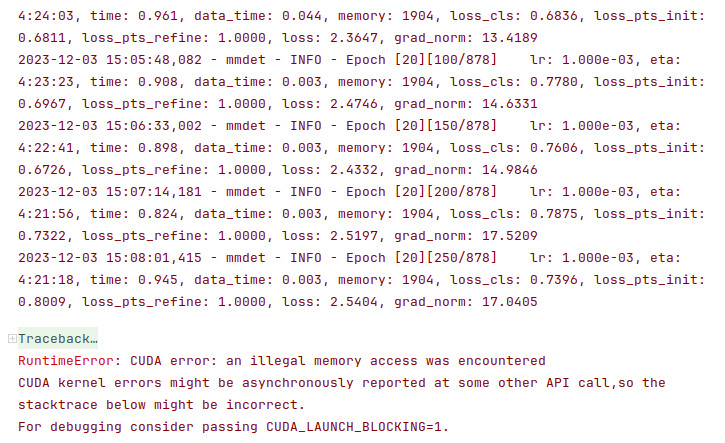
\includegraphics[width=450px]{./mmrotate8_1000p_epoch20.JPG}
		\caption{Kết quả huấn luyện khi thay thuật toán vào cả 2 hàm và chạy với dataset nhỏ.}
		\label{mmrotate8_1000p_epoch20}
	\end{center}
\end{figure} 

\begin{figure}[ht!]
	\begin{center}
		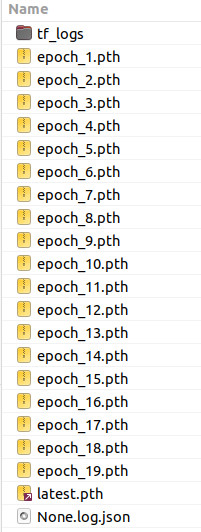
\includegraphics[width=200px]{./cau_truc_thu_muc_result.JPG}
		\caption{Cấu trúc thư muc results lưu trữ file checkpoint và file log quá trình huấn luyện.}
		\label{cau_truc_thu_muc_result}
	\end{center}
\end{figure} 

\begin{figure}[ht!]
	\begin{center}
		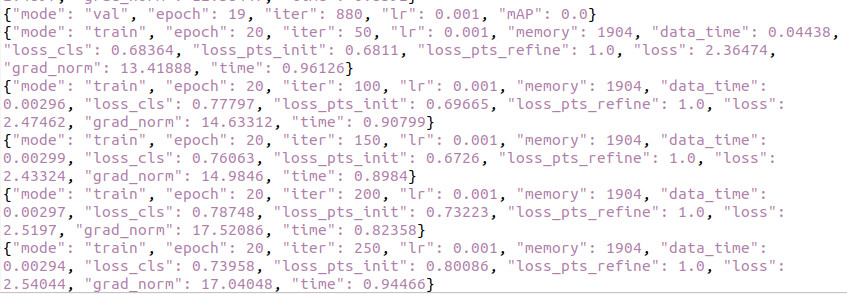
\includegraphics[width=450px]{./ket_qua_file_none_log_json.JPG}
		\caption{Một đoạn nội dung trong file None.log.json.}
		\label{ket_qua_file_none_log_json}
	\end{center}
\end{figure} 
\section{Thay thế mỗi thuật toán Jarvis và sử dụng bộ dataset nhỏ}
Do nghi ngờ kết quả lỗi xuất hiện ở hàm Jarvis\_and\_index(), em chỉ thay thuật toán vào hàm Jarvis, tức là trong quá trình huấn luyện sẽ có sử dụng cả thuật toán Jarvis March và thuật toán Outer Convex Approximation. Kết quả quá trình huấn luyện diễn ra được thuận lợi, thuật toán chạy hết được 40 epochs mà không gặp lỗi gì. Tuy nhiên do bộ dataset quá nhỏ, cùng với giới hạn các class trong dataset bị mất cân bằng nên không sử dụng được kết quả này, chỉ có thể chứng minh được là thuật toán đã hoạt động được và cho kết quả chạy chính xác. Tuy nhiên kết luận này vẫn cần phải kiểm tra và xác minh lại tính chính xác khách quan hơn. 
\chapter*{{Kết luận}}
\addcontentsline{toc}{chapter}{\vspace*{-8pt} Kết luận}

Trong quá trình làm đồ án tốt nghiệp, em đã có cơ hội được trải nghiệm chuyên ngành AI cũng như được thử sức qua các công nghệ nhận diện ảnh mới nhất. Em đã tích luỹ được những kinh nghiệm về kiến thức trong công việc cũng như các kỹ năng mềm trong xử lý các công việc liên quan đến hệ điều hành linux, cách triển khai một dự án trí tuệ nhân tạo, cách tìm hiểu thông tin từ các tài liệu chính thống.
 
Em được rèn luyện kỹ năng giải quyết các công việc con, cách tương tác với người khác để trao đổi kiến thức, từ đó rút ngắn công sức và thời gian. Đồng thời em cũng được áp dụng lại các kiến thức đã được học từ các môn trên trường vào đồ án thực tế này.





\begin{thebibliography}{30}
\addcontentsline{toc}{chapter}{\vspace*{-8pt} Tài liệu tham khảo}
	
\subsection*{Tiếng Việt}

\bibitem{FPN} Trần Văn Huy (2021), \textit{Feature Pyramid Network (FPN) Understanding}, https://huytranvan2010.github.io/Feature-Pyramid-Network/

\bibitem{DCN} Nguyễn Tiến Đạt (2022) ,\textit{tìm hiểu về Deformable Convolution Networks}, https://viblo.asia/p/tim-hieu-ve-deformable-convolution-networks-Ljy5VROb5ra
\subsection*{Tiếng Anh}

	\bibitem{Guo-Zonghao} Zonghao Guo, Chang Liu, Xiaosong Zhang, Jianbin Jiao, Xiangyang Ji and Qixiang Ye (2021), \textit{Beyond Bounding-Box: Convex-hull Feature Adaptation for Oriented and Densely Packed Object Detection} , IEEE/CVF Conference on Computer Vision and Pattern Recognition (CVPR).
	\bibitem{MMCV} MMCV Contributors (2018), OpenMMLab Computer Vision Foundation, \textit{https://github.com/open-mmlab/mmcv}
	\bibitem{MMRotate} MMRotate Contributors (2022),OpenMMLab rotated object detection toolbox and benchmark, \textit{https://github.com/open-mmlab/mmrotate}
	\bibitem{MMDetection} MMDetection Contributors (2018), OpenMMLab Detection Toolbox and Benchmark, \textit{https://github.com/open-mmlab/mmdetection}
\end{thebibliography} 
\end{document}
 
